\documentclass[oneside,11pt]{amsart}

%\usepackage{a4wide}
%\usepackage{epsfig}
%\usepackage{psfig}
\usepackage{graphicx}
\usepackage{natbib,latexsym,url,enumitem,pdfpages,multicol}
\usepackage{color}
\usepackage{wrapfig}
\usepackage[belowskip=-10pt,aboveskip=0pt]{caption}
\usepackage{threeparttable}

\captionsetup{
    justification=justified,
    margin=0pt,
    font=small}

%%%%%%%%%%%%%%%%%%%%%%%%%%%%%%%%%%%%%%%%%%%%%%%%%%%%%%%%%%%%%%%%%%%%%%%%
% Allow for the okina; thanks to:
% https://tex.stackexchange.com/questions/424535/how-to-type-a-proper-hawai%CA%BBian-%CA%BBokina

\usepackage[utf8]{inputenc}
\usepackage{newunicodechar}
%\usepackage{libertine}

\DeclareRobustCommand{\okina}{%
  \raisebox{\dimexpr\fontcharht\font`A-\height}{%
    \scalebox{0.8}{`}%
  }%
}
\newunicodechar{ʻ}{\okina}
\newcommand{\hawaii}{Hawaiʻi}
%%%%%%%%%%%%%%%%%%%%%%%%%%%%%%%%%%%%%%%%%%%%%%%%%%%%%%%%%%%%%%%%%%%%%%%%

\newcommand{\arcmin}{\mbox{$^{\prime}$}}
\newcommand{\arcsec}{\mbox{$^{\prime\prime}$}}
\newcommand{\gt}{$>$}

% Some fancy commenting
\definecolor{todo}{RGB}{200,0,0}
\newcommand{\comment}[2][todo]{{\color{#1}[[{\bf #2}]]}}

% Challenge counter
\newcounter{chalno}
\newcommand{\chal}[1]{\refstepcounter{chalno}\label{#1}}

% User commands
\makeatletter
\let\jnl@style=\rm
\def\ref@jnl#1{{\jnl@style#1}}

\def\ref@jnl#1{{\jnl@style#1}}% 
\newcommand\aj{\ref@jnl{AJ}}%        % Astronomical Journal 
\newcommand\araa{\ref@jnl{ARA\&A}}%  % Annual Review of Astron and Astrophys 
\newcommand\apj{\ref@jnl{ApJ}}%    % Astrophysical Journal ++
\newcommand\apjl{\ref@jnl{ApJL}}     % Astrophysical Journal, Letters 
\newcommand\apjs{\ref@jnl{ApJS}}%    % Astrophysical Journal, Supplement 
\newcommand\ao{\ref@jnl{ApOpt}}%   % Applied Optics ++
\newcommand\apss{\ref@jnl{Ap\&SS}}%  % Astrophysics and Space Science 
\newcommand\aap{\ref@jnl{A\&A}}%     % Astronomy and Astrophysics 
\newcommand\aapr{\ref@jnl{A\&A~Rv}}%  % Astronomy and Astrophysics Reviews 
\newcommand\aaps{\ref@jnl{A\&AS}}%    % Astronomy and Astrophysics, Supplement 
\newcommand\azh{\ref@jnl{AZh}}%       % Astronomicheskii Zhurnal 
\newcommand\baas{\ref@jnl{BAAS}}%     % Bulletin of the AAS 
\newcommand\icarus{\ref@jnl{Icarus}}% % Icarus
\newcommand\jrasc{\ref@jnl{JRASC}}%   % Journal of the RAS of Canada 
\newcommand\memras{\ref@jnl{MmRAS}}%  % Memoirs of the RAS 
\newcommand\mnras{\ref@jnl{MNRAS}}%   % Monthly Notices of the RAS 
\newcommand\pra{\ref@jnl{PhRvA}}% % Physical Review A: General Physics ++
\newcommand\prb{\ref@jnl{PhRvB}}% % Physical Review B: Solid State ++
\newcommand\prc{\ref@jnl{PhRvC}}% % Physical Review C ++
\newcommand\prd{\ref@jnl{PhRvD}}% % Physical Review D ++
\newcommand\pre{\ref@jnl{PhRvE}}% % Physical Review E ++
\newcommand\prl{\ref@jnl{PhRvL}}% % Physical Review Letters 
\newcommand\pasp{\ref@jnl{PASP}}%     % Publications of the ASP 
\newcommand\pasj{\ref@jnl{PASJ}}%     % Publications of the ASJ 
\newcommand\qjras{\ref@jnl{QJRAS}}%   % Quarterly Journal of the RAS 
\newcommand\skytel{\ref@jnl{S\&T}}%   % Sky and Telescope 
\newcommand\solphys{\ref@jnl{SoPh}}% % Solar Physics 
\newcommand\sovast{\ref@jnl{Soviet~Ast.}}% % Soviet Astronomy 
\newcommand\ssr{\ref@jnl{SSRv}}% % Space Science Reviews 
\newcommand\zap{\ref@jnl{ZA}}%       % Zeitschrift fuer Astrophysik 
\newcommand\nat{\ref@jnl{Nature}}%  % Nature 
\newcommand\iaucirc{\ref@jnl{IAUC}}% % IAU Cirulars 
\newcommand\aplett{\ref@jnl{Astrophys.~Lett.}}%  % Astrophysics Letters 
\newcommand\apspr{\ref@jnl{Astrophys.~Space~Phys.~Res.}}% % Astrophysics Space Physics Research 
\newcommand\bain{\ref@jnl{BAN}}% % Bulletin Astronomical Institute of the Netherlands 
\newcommand\fcp{\ref@jnl{FCPh}}%   % Fundamental Cosmic Physics 
\newcommand\gca{\ref@jnl{GeoCoA}}% % Geochimica Cosmochimica Acta 
\newcommand\grl{\ref@jnl{Geophys.~Res.~Lett.}}%  % Geophysics Research Letters 
\newcommand\jcp{\ref@jnl{JChPh}}%     % Journal of Chemical Physics 
\newcommand\jgr{\ref@jnl{J.~Geophys.~Res.}}%     % Journal of Geophysics Research 
\newcommand\jqsrt{\ref@jnl{JQSRT}}%   % Journal of Quantitiative Spectroscopy and Radiative Trasfer 
\newcommand\memsai{\ref@jnl{MmSAI}}% % Mem. Societa Astronomica Italiana 
\newcommand\nphysa{\ref@jnl{NuPhA}}%     % Nuclear Physics A 
\newcommand\physrep{\ref@jnl{PhR}}%       % Physics Reports 
\newcommand\physscr{\ref@jnl{PhyS}}%        % Physica Scripta 
\newcommand\planss{\ref@jnl{Planet.~Space~Sci.}}%  % Planetary Space Science 
\newcommand\procspie{\ref@jnl{Proc.~SPIE}}%      % Proceedings of the SPIE 

\newcommand\actaa{\ref@jnl{AcA}}%  % Acta Astronomica
\newcommand\caa{\ref@jnl{ChA\&A}}%  % Chinese Astronomy and Astrophysics
\newcommand\cjaa{\ref@jnl{ChJA\&A}}%  % Chinese Journal of Astronomy and Astrophysics
\newcommand\jcap{\ref@jnl{JCAP}}%  % Journal of Cosmology and Astroparticle Physics
\newcommand\na{\ref@jnl{NewA}}%  % New Astronomy
\newcommand\nar{\ref@jnl{NewAR}}%  % New Astronomy Review
\newcommand\pasa{\ref@jnl{PASA}}%  % Publications of the Astron. Soc. of Australia
\newcommand\rmxaa{\ref@jnl{RMxAA}}%  % Revista Mexicana de Astronomia y Astrofisica

%% added feb 9, 2016
\newcommand\maps{\ref@jnl{M\&PS}}% Meteoritics and Planetary Science
\newcommand\aas{\ref@jnl{AAS Meeting Abstracts}}% American Astronomical Society Meeting Abstracts
\newcommand\dps{\ref@jnl{AAS/DPS Meeting Abstracts}}% American Astronomical Society/Division for Planetary Sciences Meeting Abstracts



\let\astap=\aap 
\let\apjlett=\apjl 
\let\apjsupp=\apjs 
\let\applopt=\ao 



\DeclareRobustCommand{\gtrsim}{%
\mathrel{\hskip-.5em\begin{array}{c}>\\[-8pt]\sim\end{array}\hskip-.5em}}
\DeclareRobustCommand{\lesssim}{%
\mathrel{\hskip-.5em\begin{array}{c}<\\[-8pt]\sim\end{array}\hskip-.5em}}


\pretolerance=10000
\textwidth=6.4in
\textheight=8.95in
\voffset = 0.in
%\voffset = -0.3in  % For my printer
\topmargin=0.0in
\headheight=0.00in
\hoffset = 0.0in
%\hoffset = 0.33in  %  For my printer
\headsep=0.00in
\oddsidemargin=0in
\evensidemargin=0in
\parindent=2em
\parskip=0.2ex
 
\renewcommand{\baselinestretch}{1.03}

\special{papersize=8.5in,11in}

\newcommand{\markus}{\textcolor{green}}

\setlength{\parskip}{0.6 ex plus 0.4ex minus 0.2ex} \flushbottom
\pagestyle{plain} 

\begin{document}
% \thispagestyle{empty}

\pagenumbering{arabic}

\vspace*{-1.5cm}

\centerline{\textsf {\Large FOBOS: A Next-Generation Spectroscopic Facility}}
\centerline{\textsf {\large Response to Astro2020 Request for Information}}

\setcounter{page}{1}

\section*{Executive Summary}

% - Summarize your science objectives and your technical implementation at
%   a high level.

\noindent{\bf Science objectives:} FOBOS, the Fiber-Optic Broadband
Optical Spectrograph, is a facility-class, general-purpose
spectrograph for the 10m Keck II telescope. It emphasizes UV
sensitivity (up to the atmospheric limit), high multiplex, multiple
focal-plane sampling formats, and near Poissonian-level performance
over extremely long ($\sim$100 hr) integration times. Its flexible
position system enables advanced techniques for merging multiple
observing programs, including a constant fraction of fibers (5-10\%)
allocated to the full US community amounting to $\sim$100,000
fiber-hours per year. This establishes FOBOS's uniqueness, both in
term of functionality and access, among the suite of spectrographs
coming online for 8-10m class telescopes in the next decade. FOBOS is
specifically built to enable the deep spectroscopic follow-up of
upcoming large-scale imaging surveys (LSST, WFIRST, and Euclid)
identified as a significant need of the astronomy community in the US
and beyond. For example, capitalizing on the combined $\approx$\$4B
the US is investing in these imaging surveys, FOBOS can increase
LSST's dark-energy figure-of-merit by 40\% \citet{newman15}.

\smallskip

\noindent{\bf Technical implementation:} FOBOS is a fiber-fed,
fixed-format spectrograph. Its primary systems include (1) a
compensating lateral atmospheric dispersion corrector (CLADC), (2) a
robotic fiber-positioning system based on AAO's Starbug technology,
(3) micro-assembly fore-optics required to optimally couple the Keck
II input beam to the fiber feed, (4) 10m-long fiber trains that
provide at least three focal-plane sampling options (single fibers,
multiple small IFUs, and a single large-format IFU), and (5) a bank
of three 4-channel spectrographs that provide a simultanous spectral
range of 0.31-1 $\mu$m at a resolution of $R\sim3500$ across the full
band.

\smallskip

% - Summarize the technology maturity of your implementation, listing the
%   demonstrated technologies and the technologies requiring development.

\noindent{\bf Technological maturity:} FOBOS is nearing the end of
its conceptual design phase, and will begin its preliminary design
phase in Oct 2020, contingent on funding. Components of this document
represent significant improvements in FOBOS's design since the
completion of our Astro2020 submission. Although requiring
significant design work, FOBOS's backend systems are built on
well-established technologies: FOBOS's spectrographs and fiber train
inherit significantly from SDSS, MaNGA, and DESI designs. FOBOS's
front-end leverages the more than 15 years of development of the
Starbugs position system, which have been deployed and are in the
final commissioning stages for the TAIPAN instrument on the AAT.
Further development of the Starbugs technology is needed for use in
FOBOS; however this represents a 2nd-generation implementation of the
technology and will leverage simultaneous development of the
GMT/MANIFEST instrument. Further development of the micro-assembly
fore-optics is also critical; prototypes are currently being
developed with potential industry partners and tested at UCO/UCB.

\smallskip

% - Summarize areas where the data to support this RFI are not currently
%   available.

\noindent{\bf Limitations of this RFI:} Given this early stage in
development, particular project components with limited extant
data/information to address this RFI are as follows:

\newpage

\section{Science}

% - Briefly describe the scientific objectives and the most important
%   measurements required to fulfill these objectives. Feel free to refer
%   to science white papers or references from the literature.

FOBOS, the Fiber-Optic Broadband Optical Spectrograph, is a
facility-class, general-purpose spectrograph for the 10m Keck II
telescope. Although its scientific use is expected to be very broad,
FOBOS meets an explicit need of the astronomy community in the era of
deep imaging surveys, like LSST, WFIRST, and Euclid, allowing for
highly efficient follow-up spectroscopy of faint sources using one of
the world's largest telescope. The design of the instrument reflects
this need by emphasizing high target densities, multiple focal-plane
sampling formats, blue sensitivity, and a stabilized and
well-calibrated instrument performance. To help establish these
requirements, we have outlined three ``design-reference'' key science
programs that facilitate the definition of FOBOS's instrument
requirements. These key programs are:

\smallskip

\noindent{\bf (a) Dark Energy}: Distance measurements for the
billions of sources in deep-imaging campaigns, like LSST, WFIRST, and
Euclid, will hinge on the use of photometric redshifts (photo-$z$s).
FOBOS observations that target $\sim$15k sources with $24 > i_{\rm
AB} > 25.3$ in specific regions of galaxy color space \citep[see][]{masters15, masters19} can dramatically improve the photo-$z$
accuracy applied to the full LSST sample, equivalent to an {\em
increase of LSST's dark energy figure-of-merit by 40\%} \citep{newman15}. The {\it key instrument requirements} derived
from this program are (1) the blue wavelength coverage (down to the
atmospheric limit) to eliminate the usual "redshift desert", (2)
long-term stability of the instrument to allow for
near-Poisson-limited data reduction for ultra-deep, $\sim$100-hr
integrations, and (3) high multiplex to meet the target-density needs
of sources to $i_{\rm AB} > 25.3$ ($\sim$40 per arcmin$^2$).

\smallskip

\noindent{\bf (b) The baryonic ecosystem of galaxies at cosmic high
noon}: Mapping the crucial link between galaxies at $z\sim$2--3 and
the extended gas reservoirs, diffuse halos, and streaming filaments
that dominate the mass and regulate galaxy evolution in these
environments requires an instrument like FOBOS, even in the era of
JWST and ELTs. Its deep sensitivity and high sampling density enables
comprehensive tomographic reconstruction of the intergalactic medium
(IGM) across the largest cosmic structures in a single pointing
($\sim$10 transverse Mpc at $z \sim 2.5$). Its blue sensitivity
probes Ly-$\alpha$ across the complete formation epoch ($z =
1.5$--3.5) and opens access to high-ionization transitions that
reveal diffuse gas \emph{in emission}, such as O VI (1032 \AA).
Finally, its ability to combine single-fiber and multiplexed IFU
observations allows us to map the density and dynamical state of
diffuse gas at all relevant scales from the IGM to the circumgalactic
medium (CGM). The {\it key instrument requirements} derived from this
program parallel those from our ``Cosmology'' program, and
additionally require an integral-field mode that provides
two-dimensional kinematic data.

\smallskip

\noindent{\bf (c) The chemodynamical history of M31}: Compared to
existing and forthcoming spectrographs (e.g., PFS, MSE), FOBOS's high
sampling density and IFU modes offer unique capabilities for
efficiently mapping the high-source-density M31 disk. Building on
previous imaging \citep[PHAT][]{phat} and spectroscopy \citep[SPLASH][]{splash} FOBOS will provide high-S/N spectra of $\sim$100k M31
disk stars that connect [Fe/H] and [$\alpha$/Fe] patterns to the
underlying dynamics. FOBOS will use integral-field observations of
$\sim$150 young stellar clusters that yield their present-day mass
function. Additionally, a few larg-scale star-formation complexes are
observed with FOBOS's monolithic IFU (FOV $\sim$ 700 arcmin$^2$)
allow for comparison of the local star-formation activity with the
Milky Way. In general, integral-field observations of the M31 disk
enable unique background-subtraction techniques that more accurately
remove the underlying diffuse M31 light, unavailable to single-fiber
observations. Combining these FOBOS observations with integral-field
data from the SDSS-V Local Volume Mapper and PFS/MSE surveys of halo
structure, a complete picture of the Andromeda system's formation
history will address key questions about disk evolution, dwarf
galaxies, and dark matter substructure with a level of statistical
power that has so far been limited to the Milky Way. The {\it key
instrument requirements} derived from this program parallel our
previous programs and additionally motivate the monolithic
integral-field unit.

~\comment{discuss community access here?}

Beyond the scope and requirements of these ``design reference''
programs, {\bf FOBOS enables a broad range of observations}, e.g.:
Milky Way and M31 halo stars and substructure; the Milky Way bulge;
globular clusters; variable stars from cadenced LSST imaging; dwarf
galaxies; rapid time-domain followup with an always-ready IFU;
structure of Coma and Virgo galaxies with IFUs and using globular
clusters and PNe as tracers; large IFU samples at $z \sim 1$ of 2D
emission-line kinematics; galactic winds; radial stellar-population
trends from stacked spectra at $z \sim 1$; environmental group
identification at $z \sim 1$--2; galaxy cluster and proto-cluster
followup; QSO light echos in the IGM; and redshift calibration of LBG
samples at $z = 1.5$--5 for CMB lensing cross-correlation.

Finally, given the wealth of photometric data and the continued
increase in sophistication and broad application of state-of-the-art
machine-learning techniques, we expect a common theme of FOBOS
observations to be the build-up of optimized training samples. We
have already seen the power of the combination of large samples of
photometric or low-spectral-resolution data with higher resolution
training sets in inferring higher-order properties. Examples include
stellar parameters (age, metallicity, $\log g$, $T_{\rm eff}$) and
distance (e.g., Ting et al. 2018a,b) and emission-line fluxes in
galaxy spectra (e.g., Capak).

% - Of the objectives, which are the most demanding? Why?
% - Present the highest-level technical requirements (e.g. spatial and
%   spectral resolution, sensitivity, timing accuracy) and their relation
%   to the science objectives.

\subsection{Top-level Requirements}

Table \ref{tab:reqs} presents the top-level requirements for FOBOS as
they stand at the time of this writting; however, we caution that
these are still under development.

\begin{table}[h!]
\centering
\begin{threeparttable}
\caption{FOBOS Top-Level Requirements}
\footnotesize
\begin{tabular}{| l | c | p{2.5cm} | p{1.5cm} | p{4cm} |}
\hline
{\bf Description} & {\bf ID} & {\bf Requirement} & {\bf Goal} & {\bf Justification} \\
\hline
\hline
Field of View & TOP.REQ.A01 & $D=17\arcmin$ & $D=20\arcmin$ & Maximum FoV matches full Keck-Nasmyth FoV \\
\hline
MOS-fiber multiplex & TOP.REQ.A02 & 1800 &  & Achieve density of 6 arcmin$^2$ for $20\arcmin$ FoV \\
\hline
MOS-fiber aperture & TOP.REQ.A03 & $0.7\arcsec < D < 1.3\arcsec$ &  & Optimize S/N of extracted spectra given WMKO seeing distribution \\
\hline
Calibration mini-IFUs & TOP.REQ.A10 & 12 7-fiber bundles & & Flux calibration fidelity; four per spectrograph (Yan et al. 2016) \\
\hline
MOS-IFU size & TOP.REQ.A04 & $\gtrsim$5\arcsec &  & Cover scales of $\gtrsim$20 kpc at $z=2-2.5$ \\
\hline
MOS-IFU sampling & TOP.REQ.A05 & $\lesssim$0.8\arcsec & & Optimize extended-source spectroscopy \\
\hline
MOS-IFU multiplex & TOP.REQ.A06 & 45 & & 37 fibers per IFU, 15 IFUs per spectrograph \\
\hline
Monolithic IFU FoV & TOP.REQ.A11 & $D\sim$30\arcsec & & Maximum size for full fiber complement in a single IFU \\
Wavelength coverage & TOP.REQ.A07 & 0.31 - 1 $\mu$m & & Eliminate redshift desert \\
\hline
Spectral Resolution & TOP.REQ.A08 & $R = 3500$ & & Subtraction of night-sky lines in the red \\
\hline
Throughput & TOP.REQ.A09 & $\gtrsim$30\% over 95\% of the bandpass & & Competitive with other upcoming instruments \\
\hline
\end{tabular}
\begin{tablenotes}
\item MOS-IFU requirements above are optimized for the CGM science
case; however, we expect additional IFU modes to be explored,
including those that critically sample the median Keck seeing
(0.6\arcsec) and those that take advantage of a GLAO mode when it is
available at Keck.
\end{tablenotes} 
\label{tab:reqs}
\end{threeparttable}
\end{table}

The most demanding aspects of our design-reference science programs
on FOBOS's performance and instrument requirements are in its ability
to reach near-Poisson level performance for very long integrations
($\gtrsim$100-hr). Analysis of existing data from the MaNGA/SDSS-IV
survey, a survey and instrument not meant to enable such long
exposures, demonstrates a sky-subtraction fidelity of $\sim$0.2\%
(Childress et al. 2017, MNRAS, 472, 273; Bundy et al., in prep; Gu et
al.). Early commissioning data for DESI shows similar performance. A
key aspect of our design and instrument simulation work during the
instrument design phases will be to (re)assess the instrument,
calibration, and data-reduction-software systems with respect to
their expected performance over very long integration times. This
work will continue to inform the relevant system requirements well
into final design. Deviations from Poisson performance would lead to
longer integration times for our Cosmology and CGM programs; however,
the performance of current fiber-based instruments is such that we do
not expect these deviations to be significant enough to render these
programs infeasible.

% - For each performance requirement identified, describe as
%   quantitatively as possible the sensitivity of the science objectives
%   to achieve the requirement.  If you fail to meet a key requirement,
%   what would be the impact on achieving the science objectives?

\section{Enabling Technology}
\label{sec:tech}

% - Please provide information describing new enabling technologies
%   required for activity success.

There are no fundamentally new technologies needed to enable the
FOBOS concept to be realized. However, there are a few key
technologies that require new design innovations or modifications of
existing designs for there specific use in FOBOS.

% driven by low-risk

% LRS2 microlens arrays, full re-imaging system (very hard alignment problem, but lots of real-estate; PFS has microlens on the fiber, but bonded)  Need for airgap, Starbugs packaging

FOBOS's conceptual design includes fused-silica etched (FSE) gratings
in each channel of our 4-channel spectrographs. To date, FSE gratings
have had limited use in astronomical instruments; however, FSE
grating advancement has come quickly on the heels of development of
e-beam lithography techniques, which allow shaping of grating grooves
to nanometer precision. Custom designed gratings promise high
efficiency over our entire wavelength range. In particular, their use
in FOBOS overcomes a lack of volume-phase holographic (VPH) gratings
with good transmission at wavelengths shorter than 350 nm.
Prototyping and testing of these diffractive optics will be ongoing
during our preliminary design phase. If necessary, our design can be
rescoped to use VPH gratings with appropriate compensations to the
rest of the design given their limitations.

Additional key design elements are:
%
\begin{enumerate}
\item Implementation of a compensating lateral atmospheric dispersion
corrector (CLADC) that includes a fold mirror between its 2nd and 3rd
elements. The mirror folds the incoming beam such that the face of
the final element of the CLADC is perpendicular to the gravity vector
and serves as the drive surface for the Starbugs positioning system
(see below). This orientation dramatically decreases the risk of
Starbug adhesion failures on the drive surface.
\item Development and process testing of micro-assembly foreoptics
composed of single lenses for single-fiber apertures and microlens
arrays for integral-field apertures.
\item Integration of both single-aperture and multi-aperture arrays
assemblies in the Starbugs piezo assembly.
\item Roughly an order-of-magnitude increase in the number of Starbugs
simultaneously used in a positioning system.
\end{enumerate}

% - Please indicate any non-US technology required for activity success
%   and what back up plans would be required if only US participation
%   occurred. 

\subsection{Non-US Technologies}
\label{sec:starbugs}

The fused-silica etched gratings in our current design are a
proprietary technology of the Fraunhofer Institute for Applied Optics
and Precision Engineering (IOF) in Germany. The IOF produce the most
efficient FSE gratings in the world, as needed for the unique
sensitivity requirements for FOBOS and particularly in its UV channel
(see above).

The FOBOS robotic focal-plane positioning system uses the Starbugs
technology, developed exclusively by Australian Astronomical Optics
at Macquarie University in Sydney, Australia. No similar technology
exists from a US vendor or otherwise. The Starbugs technology is very
attractive for FOBOS for three reasons: (1) It has the potential to
allow for multiple focal-plane modules specifically designed with an
exchange procedure that can be performed during daytime telescope
operations. (2) Similarly, the system allows for upgrade paths that
add new focal-plane sampling modes/modules that either interface with
the currently proposed FOBOS spectrographs or new spectrographs that
provide expanded capabilities (e.g., higher spectral resolution). (3)
Starbugs allow for the very large patrol radii needed for the
mini-IFU modes, in particular.

Starbugs are currently deployed by the TAIPAN instrument on the
Anglo-Australian Telescope (AAT). TAIPAN's commissioning phase has
proven critical to the refinement of the Starbugs design, and the
instrument is nearly ready to enter normal operations. AAO is deeply
invested in the future of the Starbugs technology, both via our
interest in their use in FOBOS, but also via their development of
MANIFEST, a front-end for the first-light spectrographs built for the
Giant Magellan Telescope.

In the event that the Starbugs technology becomes untenable for
implementation in FOBOS, we will explore zonal position systems
similar to those used by DESI, PFS, and SDSS-V. This may require a
descope of the number of focal-plane sampling modes available or
exploration of other technologies that may enable these modes, such
as highly efficient fiber switching.

% - For any technologies that have not been demonstrated by sub-scale or
%   full-scale models as of this request, please describe the rationale
%   for your technical maturity assessment, including the description of
%   analysis or hardware development activities to date, and its
%   associated technology maturation plan.
% TODO: Come back to this.

% - Describe the aspect of the enabling technology that is critical to the
%   concept’s success, and the sensitivity of mission performance if the
%   technology is not realized or is only partially realized.
% TODO: Assess the sensitivity of FOBOS to each of the technologies listed above?

% - Provide cost and schedule assumptions by year for all development
%   activities, and the efforts that allow the technology to be ready when
%   required, as well as an outline of readiness tests to confirm
%   technical readiness level.
% TODO: Just refer to the cost section?

\section{Telescope}

FOBOS is an instrument planned for the existing Keck II telescope.
Installation, integration, and commissioning of the instrument are
minimally described in our work breakdown structure (see Section
\ref{sec:cost}), with specific details to be worked out in
consultation with our Keck partners during our upcoming preliminary
design phase.
 
% These details are irrelevant to FOBOS:
% - Provide an overview description of the characteristics and
%   requirements of the optical telescope(s), antenna(s), or collector(s)
%   highlighting key capabilities and any residual technology risks. 
% - Provide diagrams or drawings showing the observatory or antenna array
%   with the instruments and other components labeled and a descriptive
%   caption.
% - Please provide any available review packages (e.g. Conceptual Design
%   Review, Preliminary Design Review) that describe the scope of
%   technical design and implementation.
% - Please describe any hardware/software with significant heritage.
% - Please fill out the table below regarding the primary scientific
%   equipment (e.g., Telescope or Antenna Array). Expand, contract, or
%   modify this table as necessary and applicable.
% - Identify and describe the three components of lowest technical
%   maturity, and explain how and when these components will be
%   demonstrated in hardware.
% - What are the three greatest risks to cost, schedule, and performance?
% - Describe any aspect of the design or implementation that may require
%   non-US participation.

\section{Instrumentation}

\begin{figure}[h!]
\vskip -0.1in
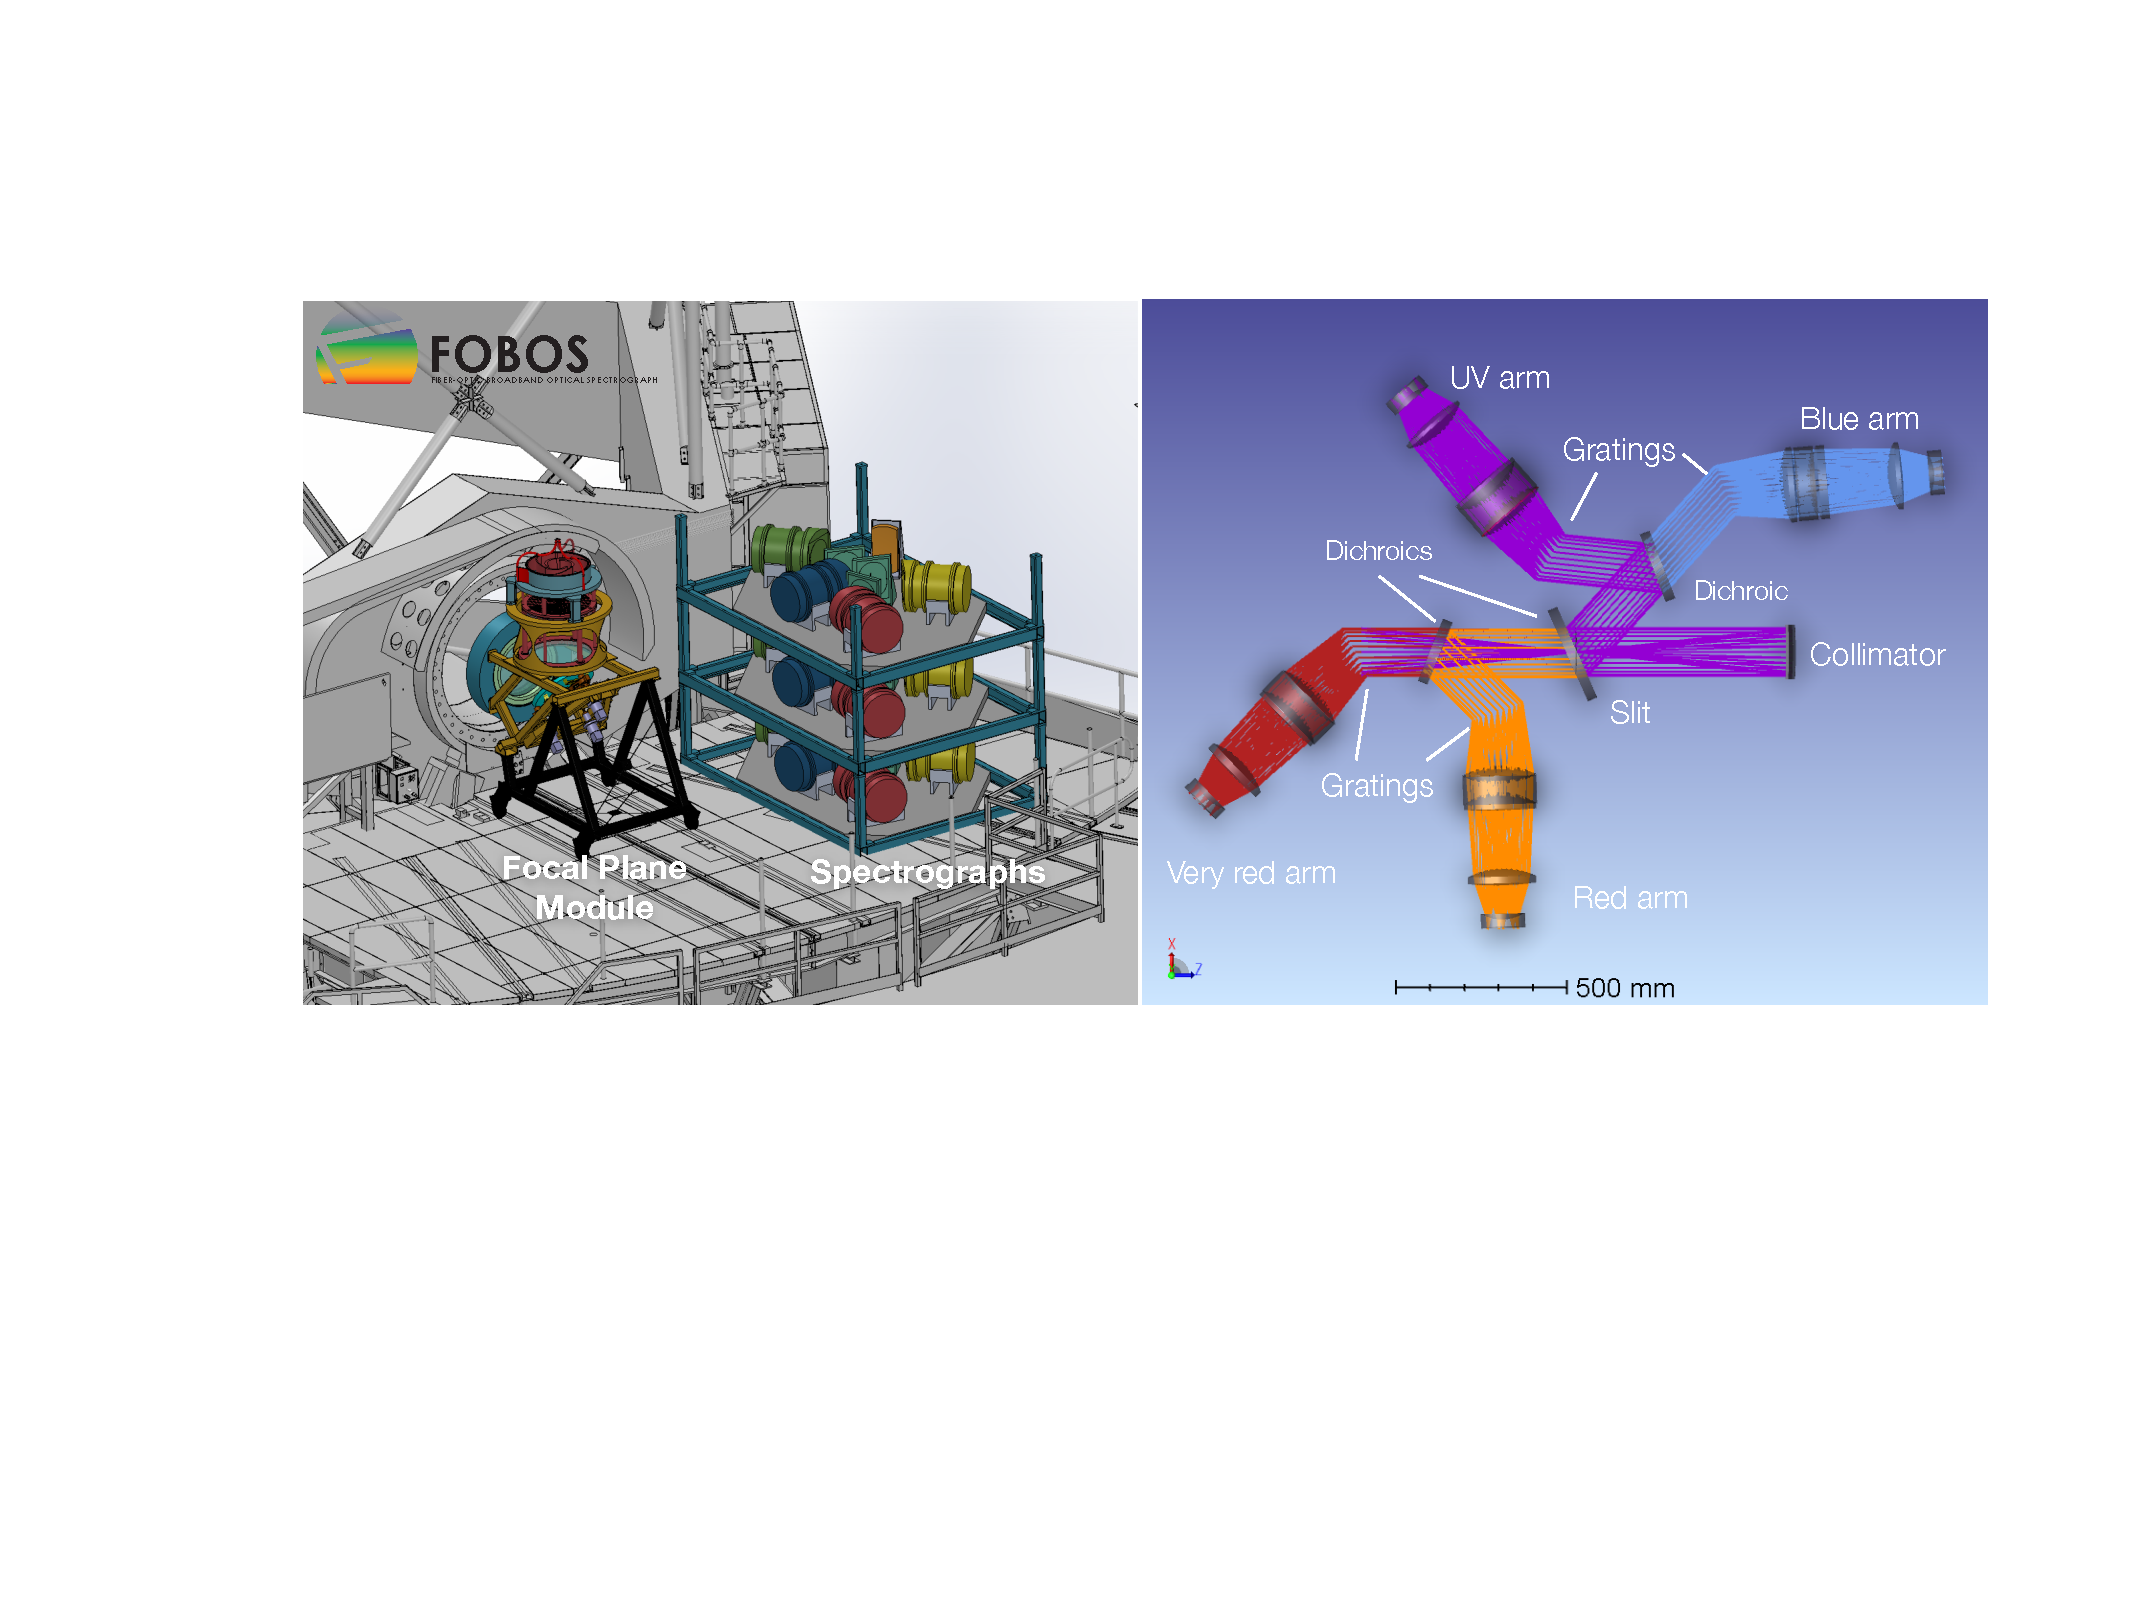
\includegraphics[width=\textwidth]{FOBOS_inst_2019-10-28.pdf}
\caption{\small {\it Left}: Rendering of FOBOS instrument systems
deployed at the Keck II Nasmyth port. {\it Right}: Optical layout of
one of the three four-armed FOBOS spectrographs.}
\label{fig:layout}
\end{figure}

% - Describe the proposed science instrumentation, and briefly state the
%   rationale for selection. Discuss the capabilities of each instrument
%   (Inst #1, Inst #2 etc.) and how the instruments are used together.
%   Indicate whether cryogens or other cooling are required. 

% - Briefly describe any concept, feasibility, or definition studies
%   already performed and please provide any available Review Packages
%   (e.g., Conceptual Design Review, Preliminary Design Review) that
%   describe the instrument and its design and implementation.

The current conceptual design of FOBOS inherited much from the
concept of a fiber-based optical spectrograph for the Thirty-Meter
Telescope in a trade/down-selection study for its Wide-Field Optical
Spectrograph (WFOS). FOBOS is still in its conceptual design phase,
and therefore no CDR package has yet been produced or included in
response to this RFI.

% - What are the three primary technical issues or risks?
% - Describe any instrumentation that may require non-US participation. 

The current conceptual designs for all FOBOS sub-systems are briefly
described in the following subsections, with its instrument
specifications summarized in Table \ref{tab:instrument}. We also
briefly comment on the technical maturity and heritage of the
components within each sub-system. Our risk register assigns the
{\bf three highest risk levels} to:
%
\begin{enumerate}
\item the performance (uniformity and stability) of our calibration
system and calibration procedures,
\item the Starbugs positioning system (the only system provided by a
non-US partner; see Section \ref{sec:starbugs}), specifically
adhesion and fine-position control, and
\item the micro-assembly fore-optics, specifically the manufacturing,
assembly, and alignment process control.
\end{enumerate}

\begin{wrapfigure}{r}{0.35\textwidth}
\small
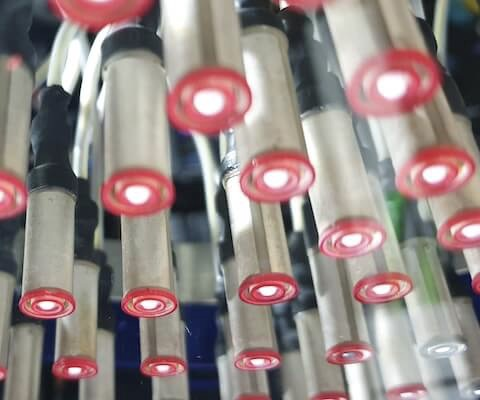
\includegraphics[width=0.35\textwidth]{starbugs_v1.jpg}
\caption{Starbugs mounted at the focal plane of the AAT. Light
enters from the image bottom, where the red or gray
``slipper'' of each Starbug contacts a field plate and is adhered to
it via a leaky vacuum. Each Starbug houses
a single-fiber aperture (white). For FOBOS, the contact surface will be
an optical element of the CLADC, always perpendicular to the
gravity vector, and the Starbugs will be adapted to hold either a
single-aperture microlens assembly or an integral-field microlens
array.}
\label{fig:org}
\end{wrapfigure}

\subsection{Focal-Plane Module}

Light from the Keck II telescope Nasmyth port (Fig \ref{fig:layout};
left) passes through the first two 946mm-diameter lenses of a 3-lens
CLADC before encountering a 45$^\circ$ mirror that folds the beam
vertically upwards. The third lens of the CLADC is horizontal with
the surface always perpendicular to the gravity vector. Positioned at
the focal plane of the telescope$+$CLADC optics, this also serves as
the mounting surface for downward-pointing Starbugs. The risk of
Starbug adhesion loss and focal-plane coupling failure is
significantly reduced by using a horizontal mounting surface
($20\arcmin$ diameter). The mounting surface rotates to match the
field rotation of the telescope as it tracks the sky. Each Starbug
patrols zones of up to several arcminutes and can be placed as close
as 10\arcsec. Three back-illuminated fibers embedded in the housing
of each Starbug are combined with a fast, imaging metrology camera
that enables reconfiguration times of as little as 2 minutes. See
Section \ref{sec:starbugs} for a discussion of their heritage,
maturity, and advantages.

\subsection{Focal-Plane Sampling \& Robotic Positioning System}

Microlens fore-optics coupled to each fiber demagnify and speed up
the telescope beam from $f/15$ to $f/5$. This provides better
coupling of the fiber to the telescope beam --- minimizing losses
from focal-ratio degradation --- and provides an $0.8\arcsec$ on-sky
diameter of each fiber. Integral-field observations are accomplished
by coupling large-fill-factor microlens arrays to fiber bundles. Team
members have experience with microlens coupling to fibers
(SDSS-III/APOGEE) and we are currently prototyping microlens optics
and optomechanical assemblies for lab and on-sky testing. Lab testing
is being performed at both UCO and UCB/SSL, and we are exploring
partnerships for the at-scale manufacturing of these components.

Separate Starbug designs will be produced to house either the
single-fiber or integral-field assemblies. These Starbugs will be
incorporated into separate modules that are stored outside the focal
plane and can be exchanged with the module attached to the focal
plane via a day-time procedure. This allows FOBOS to switch between
different fiber suites: 1) individual fibers, 600 per spectrograph;
2) A set of 15 multiplexed fiber-bundle IFUs (per spectrograph), each
composed of 37 fibers and spanning up to 5.6\arcsec; 3) A
30\arcsec-wide monolithic IFU\footnote{This mode would be unique at
Keck. Compared to KCWI+KCRM, FOBOS's monolithic IFU will emphasize
FoV over spatial resolution and blue sensitivity. KCWI+KCRM covers
0.36--1.0 $\mu$m and to achieve $R \sim 3600$ over the full bandpass,
KCWI+KCRM reduces its FoV to 8.4 $\times$ 20.4 arcseconds, an area
5$\times$ smaller than the FOBOS monolithic IFU.} (1641 fibers). In
all cases, $\sim$10\% of individual fibers are reserved for sky
sampling and 5--10 mini-bundles (7 fibers) observe stars in the field
for flux calibration and PSF monitoring.

Current designs for both the mini-IFUs and the monolithic IFU flow
from our science requirements; however, we are still exploring other
possible modes, enabled by the flexibility of the Starbugs
positioning system and focal-plane module design. In particular, our
design will accept and take advantage of ground-layer adaptive optics
(GLAO) corrections from an anticipated GLAO system at Keck II. GLAO
improves depth, enables crowded source targeting, and opens new
science territory through spatially-resolved galaxies beyond
$z\sim0.5$. Particularly for the latter, we would expect to deploy an
IFU mode that critically sampled the improved GLAO PSF.

\subsection{Fiber-feed \& Spectrographs}

Three spectrographs are mounted on the Nasmyth deck and connected to
the adjacent focal-plane module (Fig \ref{fig:layout}; right) via a a
short ($< 10$m) fiber run (not pictured) in order to preserve UV
throughput (cf., the much longer fiber runs for prime-focus
instruments, such as Subaru-PFS and DESI). Stress-relief features in
the cabling reduce focal-ratio degradation. Our team has significant
experience with fiber-fed spectrographs, drawing from SDSS and DESI
heritage.

Each of the three spectrograph uses dichroics to divide the 140 mm
diameter collimated beam into four wavelength channels with combined,
instantaneous coverage from 0.31--1 $\mu$m. High-efficiency
fused-silica etched (FSE) gratings provide mid-channel spectral
resolutions of $R \sim 3500$ for all channels. The spectrographs use
$f/2.25$ refractive cameras and 6k$\times$6k, 15 $\mu$m-pixels CCD
detectors. The camera platescale is such that the images of the
150$\mu$m fiber cores are sampled by 5 pixels in all channels. Our
spectrograph design draws significantly from the design of the DESI
spectographs.

The spectrographs are mounted in a permanent temperature-controlled
housing, providing a stable environmental temperature ($\pm$1C). Heat
rejection of electronics components in the dome is done through a
glycol cooling loop. Cyrogenic cooling of the science detectors is
provided by liquid N$_2$. The estimated end-to-end instrument
throughput peaks at 60\% and is greater than 30\% at all wavelengths.

\subsection{Calibration System}

FOBOS has a comprehensive strategy for precise calibrations, drawing
on significant heritage from purpose-built calibration systems for
SDSS, DESI, and PFS. FOBOS's calibration system is critical to its
ability to provide near-Poisson performance for very long
integrations. Specific concerns involve the stability of the fiber
input and output beams both between fibers and as a function of time
for a given fiber.

Our current concept for the calibration system and calibrations
procedures are as follows. Afternoon flat-field and arc-line
exposures will use a carefully illuminated interior dome screen,
acquired specifically for FOBOS calibrations but also as a general
good for the Observatory. Nighttime calibrations involve re-orienting
the fold mirror under the focal plane to accept light from a nearby
light source and optical assembly that mimics the telescope pupil.
Afternoon and relative fiber-to-fiber measurements from nighttime
calibrations will be combined to model the instrument$+$sky response
during observations.

\begin{table}[h!]
\centering
\caption{FOBOS Instrument Specifications}
\footnotesize
\begin{tabular}{| l | r | r |}
\hline
{\bf Item} & {\bf Value} & {\bf Units} \\
\hline
\hline
Type of instrument      & Spectrograph & \\\hline
Number of spectrographs & 3 & \\\hline
Multiplex & 1800 & single fibers \\
                        & 45 & 37-fiber IFU \\
                        & 1 & 1641-fiber IFU \\\hline
Field of view: Patrol   & 315 & arcmin$^2$ \\\hline
Field of view: Fiber    & 0.5 & arcsec$^2$ \\\hline
Field of view: Mini-IFU & 25 & arcsec$^2$ \\\hline
Field of view: Large-IFU & 705 & arcsec$^2$ \\\hline
Spectral range          & 0.31-1 & $\mu$m \\\hline
Spectral resolution     & 3500 & $R=\lambda/\delta\lambda$ \\\hline
Number of detectors     & 12 & 4 per spectrograph \\\hline
Detector size           & 6k $\times$ 6k & \\\hline
Thermal requirements    & & \\\hline
Size: Spectograph bank  & & m $\times$ m $\times$ m \\\hline
Size: Focal-plane module & & m $\times$ m $\times$ m \\\hline
Data volume (Section \ref{sec:ops})           & $<$100 & Gb \\\hline
Development Schedule    & 100 & months \\\hline
\end{tabular}
\label{tab:instrument}
\end{table}

% - Indicate the technical maturity level of the major elements and the
%   specific instrument maturity of the proposed instrumentation (for each
%   specific Inst #1, Inst#2 etc.), along with the rationale for the
%   assessment (i.e. examples of heritage, existence of breadboards,
%   prototypes, mass/volume and power comparisons to existing units, etc.
%   and any identifications of major long lead items). 

% - Describe the heritage of the instruments and associated sub-systems.
%   Indicate items that are to be developed, as well as any existing
%   hardware or design heritage.

% - Please fill out the table below regarding each instrument (if
%   applicable). Copy as needed for all instruments. Expand this table as
%   necessary and applicable.

\section{Facilities}

% - If a site is not yet selected for the project, describe the
%   anticipated approach to conducting site studies, obtaining site
%   permissions, and executing environmental impact studies.
% - Please provide any available site plans. If such plans already address
%   items 2-5 below, these items do not need to be addressed separately.
% - Describe the site and its location, including size, altitude, access,
%   number of buildings, size of building(s) footprint and volume,
%   existing infrastructure, power, internet, environmental considerations
%   and logistics (proximity to major airport, housing and support for
%   construction crews and facility staff etc.).
% - Identify which facilities will be new and which facilities may be
%   pre-existing. Describe any existing facilities and their estimated
%   remaining useful life. Describe any upgrades to existing facilities
%   that will be undertaken. Describe any anticipated shared use of site
%   facilities between the concept being proposed and existing telescopes.
% - For antenna arrays, provide specific infrastructure required such as
%   concrete pad size, communications buildings, etc. for each element in
%   the array. For telescope mirrors, describe infrastructure needed for
%   mirror maintenance, e.g. coating facilities.
% - Describe atmospheric and radio frequency interference (RFI)
%   characteristics of the site insofar as they would affect observations
%   with the concept being proposed.

\section{Operations \& Observation Strategy}
\label{sec:ops}

% - For instrument operations, provide a brief functional description of
%   operational modes, and calibration schemes. This can be documented in
%   the Operations Section. Describe the level of complexity associated
%   with analyzing the data to achieve the scientific objectives of the
%   investigation. Describe the types of data (e.g. bits, images).

FOBOS is a general-purpose, facility-class instrument that is
expected to integrate into the existing operational structure of the
W.~M.~Keck Observatory. Other instruments will share use of the Keck
II Nasmyth port used by FOBOS (e.g., KCWI), such that the focal-plane
module will be regularly rolled in and out of position, using the
rails pictured in Fig. \ref{fig:layout}. Given their size and our
emphasis on spectrograph stability, however, FOBOS's spectrographs
will be housed in a permanent, temperature-controlled stucture on the
Nasymth deck.

FOBOS emphasizes flexibility in focal plane sampling, providing
multiple focal-plane modules with different sampling options. These
modules will be stored with the spectrograph structure and exchanged
during a day-time procedure; i.e., a single focal-plane sampling
option will be used in a given night. For a given focal-plane
sampling mode, FOBOS will support various observing modes ranging
from direct, PI-led control of the system to an automated, AI-led
merging of multiple observing programs (see MAISTRO below).

% - Provide a description of the science operations. For example:
%   pre-observational planning, data processing/reduction required,
%   coordination with other facilities.
% - Summarize key software development and any science development
%   required.
% - Summarize any archiving requirements. 

\subsection{Data Management System}

FOBOS is a complex instrument, both in terms of its active hardware
systems and in how it will be used. As such, FOBOS will require a
sophisticated data management system, which governs all software
related to planning and executing FOBOS observations, as well as the
collection and processing of the resulting scientific data.
Commensurate with FOBOS's development phase, we outline this system
below. We note here that this system specifically does not include
any software related to the operation or control of the FOBOS
mechanisms or their components. Operational software is handled by a
separate WBS element. The FOBOS data-management system is broken into
five main interdependent subsystems and an overarching application
program interface (API), {\it the Manager}, that allows for
communication between these systems. These five sub-systems are:

~\comment{emphasize partners more here}

\begin{enumerate}
%
\item {\it The Doctor}: FOBOS will maintain a database of metadata
that monitors the current state of the instrument, a historical
record of the state of the site, telescope, and instrument at the
time of the observations, and figures-of-merit for the quality of the
data produced.
%
\item {\it The Producer}: FOBOS will provide a holistic software
package to plan full, multiple-pointing observing programs. This is
divided into two subsystems: (1) {\it MAISTRO}, Modular Artificial
Intelligence System for Target Reallocation and Observing, an
``artificial intelligence'' (AI) targeting system that will learn
optimization strategies for user-controlled and multi-program target
assignment, and (2) {\it the Composer}, an instrument simulation
suite that produces realistic raw data products that can be processed
through the data-reduction and data-analysis software.
%
\item {\it The Accountant}: FOBOS will provide a data-reduction
software package that provides both quick-look and science-ready,
calibrated spectra.  This system will inherit from our teams historical connection to fiber-based packages built for SDSS and DESI.
%
\item {\it The Alchemist}: FOBOS will provide an automated
data-analysis software package that provides a set of relatively
simple, high-level measurements made from the spectra (e.g.,
redshift), building on our experience with the MaNGA Data-Analysis
Pipeline.
%
\item {\it The Curator}: FOBOS will maintain an archive of all data,
from observation-specific metadata and raw detector output to reduced
and higher-level data products. This is divided into two subsystems,
the roughly static data archive provided by the Keck Observatory
Archive (KOA) and a dynamic interface and science platform for
visualization and analysis. The latter will be done in collaboration
with NSF's OIR lab and its Community Science and Data Center (CSDC).
%
\end{enumerate}


% From Keck?
% - Please provide operations plans or documents (Concept of Operations). 
% - Provide a description of the facility operations. For example: number
%   of staff required, position types, and 24-hour operation requirements.
% - Discuss observatory efficiency, e.g. the impact of maintenance and
%   engineering and calibration time on faction of science time
%   availability.
% - Describe scope of engineering activities and time (day or night)
%   needed to maintain calibration and health of telescope/array and
%   instruments.
% - Describe any high-level safety policies that will be required for
%   items of particular safety concern.

\bigskip
\section{Programmatic Issues \& Schedule}

\begin{figure}[h!]
\vskip -0.1in
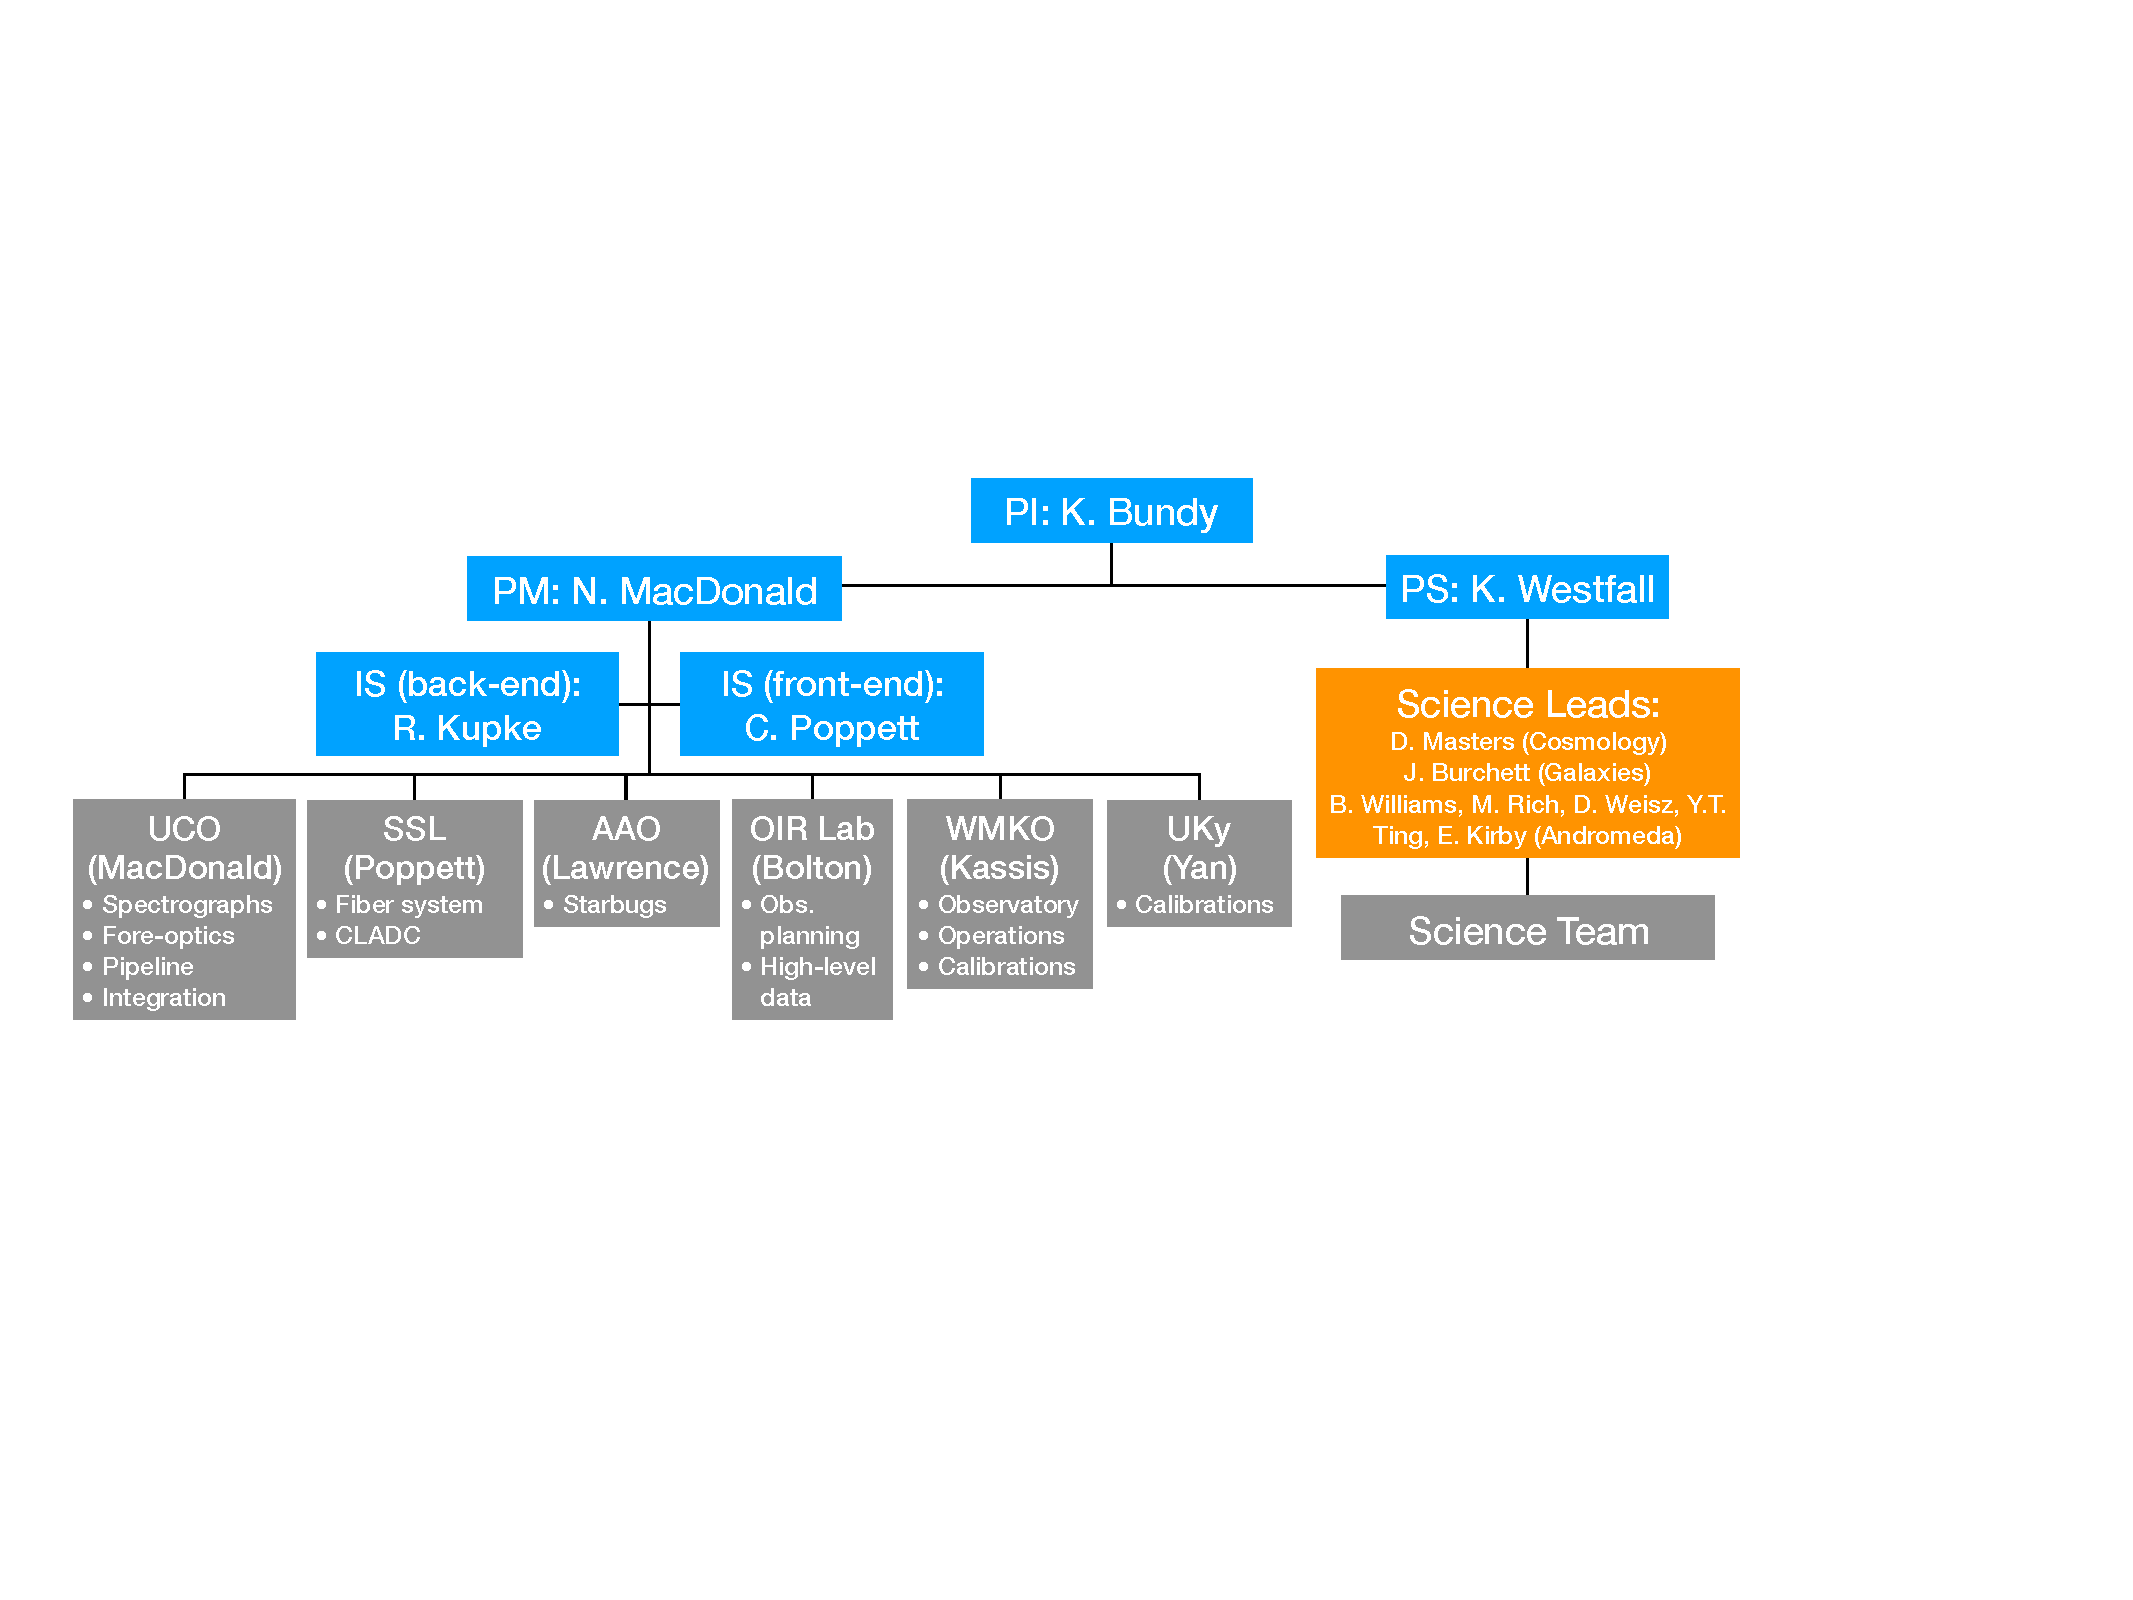
\includegraphics[width=\textwidth]{org_chart_v2.pdf}
\caption{\small FOBOS management and leadership structure.}
\label{fig:org}
\end{figure}


% - Please provide a programmatic overview that describes the structure of
%   the overall organization including any international partners or
%   university partners etc. and any money or hardware they are providing.
%   Clearly indicate schedule and costs to date highlighting what has
%   already been delivered and/or clearly capturing progress to date, if
%   applicable.

\subsection{Team Structure and Partners}

FOBOS is an international collaboration with partner institutions in Arizona, California, Hawaii, Kentucky, Pennsylvania, Washington, and Australia.  The central project office is centered at U.C.\ Santa Cruz under the University of California Observatories.  FOBOS continues to actively recruit partners and expects the collaboration will grow over time.  The organizational chart and management structure is shown in Figure \ref{fig:org}.  Each partner institution is described further below:

\medskip
\noindent{\textsf{University of California Observatories.}}  The University of California Observatories (UCO) manages a
world-renowned facility on the University of California, Santa Cruz, campus for the design, construction, and testing
of astronomical instrumentation.  With a staff of leading optical designers, engineers, and instrument scientists, UCO
has a long heritage of producing state-of-the-art instrumentation, including many spectrometers (e.g., DEIMOS), as well
as controls software for the Lick and Keck Observatories.  The recent delivery of K1DM3\footnote{K1DM3: Keck 1
Deployable Tertiary Mirror.} illustrates the close relationship between WMKO and UCO, which allows us to leverage
detailed knowledge of the observatory structure, protocols, interfaces, software and systems requirements, and
instrument deliverables.  UCO has provided significant in-kind support ($\sim$\$270k) to the FOBOS Conceptual Design effort.

\noindent{\textsf{W.~M.~Keck Observatory.}} WMKO has provided funding (\$240k in 2018-2019) as well as technical guidance for initial stages of FOBOS development and its interface to
the observatory.  FOBOS ranks as one of WMKO's top priorities in the coming decade, as encapsulated in its 2016
Strategic Plan and evidenced by its commitment to make 30 nights available to the U.S.\ community over this MSIP
proposal period as a way to deepen community involvement in Keck during the FOBOS design phase. WMKO personnel play a
key role in the proposed work through joint design of physical interfaces, safety protocols, the calibration systems,
operational modes, and software systems both for operations and data management.  Initial work has already identified
FOBOS placement and mounting options that allow it to integrate into Keck's planning for its evolving instrument suite.

\noindent{\textsf{SSL, LBNL, and DESI Fiber Lab.}} C.~Poppett serves as one of two FOBOS instrument scientists,
bringing significant expertise and facility resources from the DESI fiber system build.  Facilities developed for the
DESI fiber system include a precision optical bonding bench that facilitated the manufacture and test of 6000 fiber
optic assemblies for DESI. DESI also connected the focal plane fibers to the spectrograph slits via a custom splicing
station.  FOBOS, through a partnership with Berkeley's Space Science's Lab (SSL), will be able to utilize much of the
same lab equipment, developed expertise, detailed training documentation and procedures.

\noindent{\textsf{NSF OIR Lab.}}  NSF’s OIR Lab is an integrated national center recently created through the
combination of NOAO, Gemini, and LSST Operations. The Lab brings significant experience connecting with and serving the
U.S. astronomical community. Through an initial in-kind contribution of effort from OIR lab, FOBOS will utilize this
background in developing open-access models and community key programs. NSF’s OIR Lab is also investing significantly
in building data servicing platforms for public-facing data sets from LSST, DESI, and elsewhere.  Adapting these to
FOBOS will serve as an additional in-kind contribution. The Lab is a key partner in developing tools for science-ready
interaction with high-level FOBOS data products.

\noindent{\textsf{Australian Astronomical Observatory.}} The Australian Astronomical Optics (AAO, previously Australian
Astronomical Observatory) has worked with the FOBOS team during conceptual design to develop designs for the CLADC and
confirm the feasibility of Starbugs at the FOBOS focal plane.  The Starbugs fiber positioners have been under
development at AAO for nearly 15 years and have recently been deployed on-sky on a new instrument called TAIPAN
\cite{staszak16}.  Australian scientific interest in FOBOS is high.  AAO-Macquarie aims to leverage this interest to obtain Australian government funding to offer in-kind support for a majority of their work in FOBOS, securing Australia as a major FOBOS partner.


\noindent{\textsf{Swinburne University.}} Swinburne is a long-time Keck Observatory partner and will be prototyping micro-optics assemblies for FOBOS fibers.  Swinburne, in concert with AAO-Macquarie, is pursuing Australian ``LIEF'' funding opportunities to increase in-kind FOBOS contributions in 2020.


\noindent{\textsf{CMU \& LSST Data Science.}} The Carnegie Mellon University Machine Learning and Statistics
departments are leading institutes in the field of data science.  Project members Mandelbaum and Rau are long time
collaborators of the CMU Machine Learning department.  CMU Department of Statistics professor C.~Schafer is Co-Chair of
LSST's Informatics and Statistics Science Collaboration (ISSC).


\noindent{\textsf{UW \& LSST Operations.}} The University of Washington (UW) is an important LSST institution with significant planning, operations and data-support personnel that we will leverage for the design of similar FOBOS systems.  This not only provides valuable expertise but deepens the link between FOBOS and one of its most critical targeting data sets in LSST.


\noindent{\textsf{UC Campuses.}} UC astronomers across all campuses are contributing significant science support to FOBOS and have committed to future in-kind observing time contributions that will enable public data product delivery.  We highlight contributions from several UC astronomers.  D.~Weisz (UC Berkeley) is driving the Local Group and M31 satellites science definition and requirements.  Team member M.~Cooper (UC Irvine) lends significant expertise and resources in contributing to FOBOS survey planning and data reduction efforts.  At UCLA, M.~Rich co-leads the FOBOS Andromeda science program while A.~Shapley is involved in science program definition for $z \sim 2$ galaxy evolution studies.  At UC Riverside, B.~Siana is helping define the monolithic IFU design drivers and G.~Becker to motivating high-multiplex observations at high redshift.  J.~Hennawi (UCSB) is contributing to the IGM tomography and quasar light-echo science.  At UC Santa Cruz, J.~Burchett leads the FOBOS galaxy program while R.~Guhathurkata and C.~Rockosi are helping define the M31 survey program.  J.~Brodie, also at UCSC, is contributing to requirements definition for IFU science of nearby diffuse galaxies.

\noindent{\textsf{IPAC.}} The Infrared Processing \& Analysis Center provides in-kind support to the Keck Observatory Archive (KOA) which will serve raw and reduced FOBOS data.  IPAC is exploring cross-referencing tools to connect FOBOS planning and observations to available photometry catalogs, especially those in service of NASA missions (e.g., WFIRST).

\noindent{\textsf{Caltech.}} Team member, E.~Kirby, is a major contributor to the FOBOS M31 program definition and bridges FOBOS development with Subaru's PFS, of which Caltech is a partner.


\subsection{Progress and Initial Spending}


The FOBOS Conceptual Design is on target to complete in late 2020.  Conceptual Design has been funded by a combination
of UCO and WMKO funding.  By early 2020 FOBOS will have spent \$510k on the Conceptual Design effort. An additional
\$200--400k is expected to be made available to the team in 2020 by WMKO to complete conceptual design and provide a
bridge to the NSF funding.  Of the \$510k, \$150k has been spent on risk mitigation hardware development to help retire
the risk associated with micro-optics coupling to the fibers.  First results from this effort are expected in early
2020.  Another \$50k has been spent on community outreach and scientific workshops from 2016--2018 to help set the high
level instrumental deliverables of the instrument.  The balance of \$310k has been spent on design studies and
engineering of the FOBOS instrument.

\noindent The status of deliverables from the Conceptual Design effort are summarized below:

\begin{itemize}
%
\item Science Case Requirements Document has been drafted.  WMKO funded community engagement exercises in the initial
FOBOS design drivers in 2017.
%
\item Draft manuscript (Bundy et al., in prep) detailing fiber stability requirements and demonstrating
necessary performance based on existing instrumentation for faint-object
fiber spectroscopy on large-aperture telescopes.
%
\item Design specification documents and optical (Zemax) models for the
CLADC, lenslet fiber fore-optics, spectrograph layout, and cameras.
%
\item Vendor rough-quote estimates for the CLADC, Starbugs positioners, fiber
run, dichroics, FSE gratings, and detector
systems.
%
\item Initial SolidWorks modeling of the focal-plane module is complete.  
Vendors of focal-plane rotation and retraction systems identified.
%
\item Detailed Microsoft Project plans through Preliminary Design and
out to instrument deployment.  
%
\item Risk matrix capturing 48 risk items and scoring their probability
and consequence severity before and after mitigation strategies.
%
\end{itemize}

\subsection{Schedule Outlook}

\begin{figure}[h!]
\vskip -0.1in
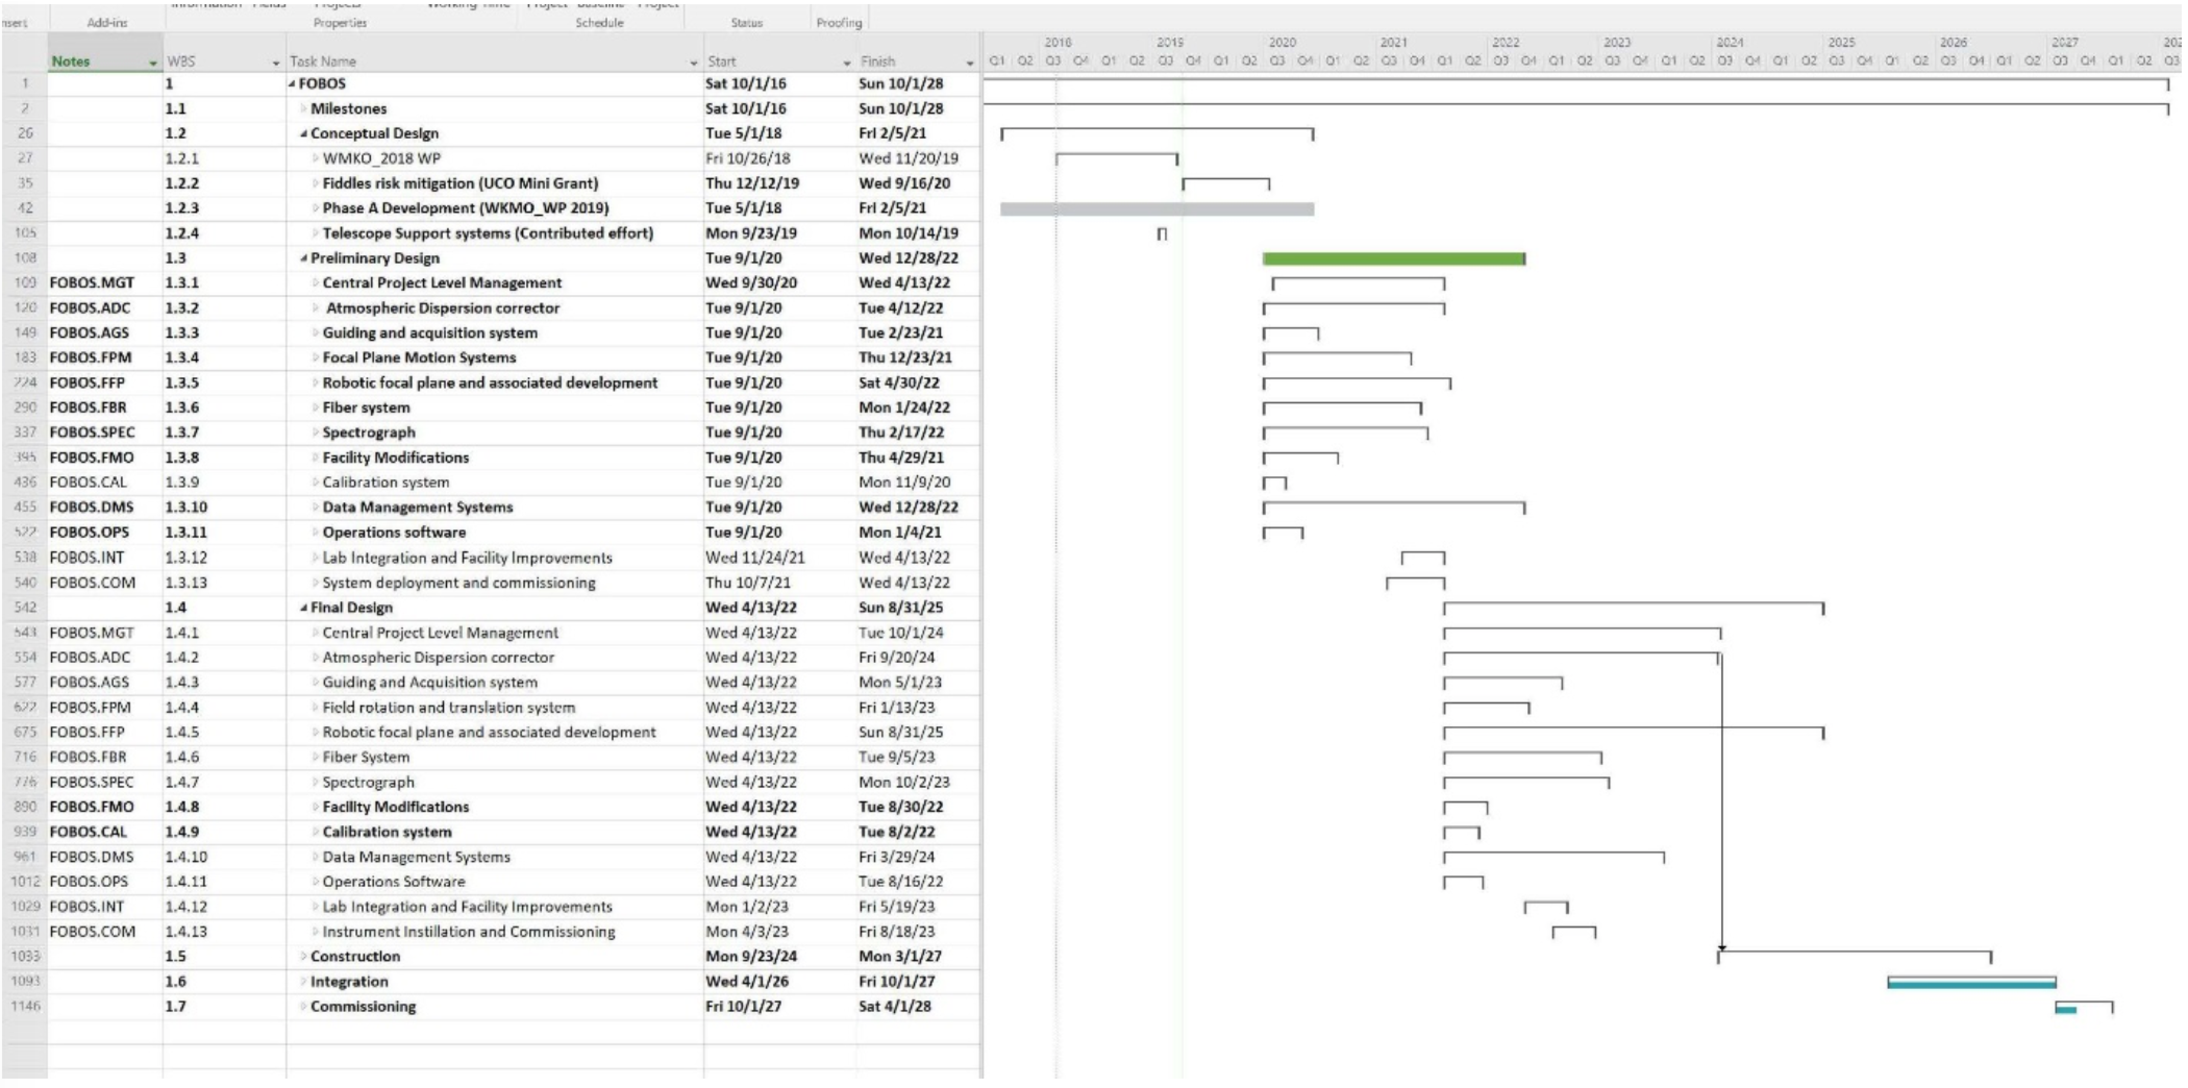
\includegraphics[width=\textwidth]{gantt_v1.pdf}
\caption{\small High-level view of the FOBOS MS Project Plan, highlighting key milestones.}
\label{fig:gantt}
\end{figure}


If our 2020 NSF MSIP proposal is successful, effort on the FOBOS instrument is expected to ramp up in October of 2020
with a  traditional Preliminary and Final Design phase.  These phases will continue until August of 2025 and be
followed by fabrication, assembly and integration, with an first-light date of 2028.  While we are vigorously pursuing
other funding paths, delays in federal support of the project will delay the overall schedule.  
A high-level schedule is shown in Figure \ref{fig:gantt}.  

A number of procurements during construction have long lead times.  In order to reduce schedule pressure, construction will start on some sub-systems prior to completion of the final design of the overall instrument.  These
systems will be reviewed independently of the formal Final Design Review.  They include the spectrograph camera
assemblies (FOBOS.SPEC.CAM in the WBS, see below) and the Atmospheric Dispersion Corrector (FOBOS.ADC).

Similarly, integration of the instrument focal plane assembly at AAO and the spectrographs at UCO is expected to
overlap with the construction phase starting in March 2026.  Delivery to the telescope of both focal plane and
spectrograph facility are planned for October 2027.  A commissioning phase is expected to end in April 2028 after which
scientific operations would start.

This schedule is somewhat conservative as it assumes all the hardware must be complete before commissioning of the
instrument may start.  The modular nature of the system may allow for a staged deployment starting with a single
spectrograph and building up to the full three spectrograph bank.  A staged deployment could allow for up to a 6 month
flexibility in the first light date with some limited capabilities.  This strategy can be implemented to allow for
operations sooner than planned or to mitigate schedule slips.


% - Please describe any funding availability challenges and the total
%   impact it had, or may have, to cost and schedule.  Has all required
%   funding been committed?  If not, please explain.  Highlight in-kind
%   contributions in the past and planned from partners.  Clearly describe
%   what the NSF/DOE/Fed Gov funding request is and what it buys.

\subsection{Funding Strategy}

The conceptual design of FOBOS has been developed by funds provided by UCO and WMKO.  In addition to direct funding the Conceptual design, FOBOS has been helped by partner participation in instruments such as DESI, Fiber-WFOS, and SDSS project.  In the case of the spectrograph almost all of the design work UCO put into the development of Fiber-WFOS design study has been transferable to FOBOS.  These efforts account for significant in-kind effort towards the development that are not well accounted for.

\subsubsection{Funding Commitment and Challenges}

Fundraising for the Conceptual Design ($\sim$\$1M) has been successful.  However, there is still a large amount of funding to be raised for the project.  FOBOS is applying for the 2020 NSF MSIP grant seeking $\sim$\$6.2M to fund Preliminary Design effort.  If successful this would bring the total funds raised to $\sim$\$7.3M (cash and in-kind).  While the full instrument cost will be determined the next phase, it is anticipated that the $\sim$\$7.3M would represent between 15\% to 25\% of the total project cost.  An additional \$22.7M to \$42.7M will be required for FInal Design and construction funding in 2022.


The balance funding of the instrument development, construction through operations, is expected to come from a combination of government sources, privet fundraising through UCO and WMKO, and in-kind contributions from partners, specifically international partners. With anticipated in-kind and pivot funding the scale of the FOBOS construction and deployment is scoped to fit within an NSF MSIP proposal program.

FOBOS has been rather successful in raising funds for at least early design work.  All internal requests (4 proposals) have been funded.  An attempt at a larger sum of design money through the 2019 NSF MSRI call was unsuccessful. This process was helpful in development of the FOBOS science case and project plan which is anticipated to produce more competitive funding proposals moving forward.

\subsubsection{In-Kind Contributions}
~\\
OIR Lab: Should the current FOBOS MSIP proposal be successful the NSF OIR Lab has committed \$181,769 in software effort over years 2021 – 2023 for development of community access and data service.  We expect the OIR Lab to continue as a partner through the duration of the project. 

AAO: The AAO-MQ effort is currently paid by the project, however efforts are underway to convert the outer phases of construction, delivery and commissioning of the robotic positioning system to an In-kind effort. As this is a multi-institution negotiation between WMKO, UC, and AAO the final path is not known at this time.

IPAC: Negotiations are under way with IPAC to provide some level of data service development as an in-kind contribution.  

% - Please describe any unexpected challenges, key risks, and/or current
%   outstanding risks that require(d) significant mitigation which
%   affect/affected cost & schedule.
% - Describe the current top 3 risks to the development of the facility,
%   and proposed mitigation strategies. Please provide a top-level
%   schedule.

\section{Cost}
\label{sec:cost}

% - Provide a high-level facility unique Work Breakdown Structure (WBS)
%   with definitions. 


% - Fill out the cost estimate tables below using the broad bins provided.
%   Note the tables are divided into US Only and with International
%   Partners.  

% - Provide a basis of estimate for project WBS elements at the highest
%   levels (i.e., systems and major subsystems, as indicated in the cost
%   tables below), including internal overhead rates that are applied to
%   costs for labor.  Describe approach or methodology for highest cost
%   element estimates such as analogies, models, expert judgement,
%   construction bids, etc.  Describe cost assumptions made for each
%   element such as any production learning curves, labor and major
%   procurements.  Identify major subcontracted procurements and
%   associated vendors if available.  The “Prior” column is meant to be
%   actual costs incurred. 


FOBOS is currently in a conceptual design phase. Our current Work
Breadown Structure (WBS) dictionary is attached to this document.

All costing to date has focused on a detailed, robust, bottom-up
costing of preliminary design and final design phases consisting
mostly of engineering labor and some level of risk retirement
prototyping. Cost of outer stages of the project including
construction, integration, and commissioning are not well understood
at this time. A full detailed cost of the project is expected to be
reached before our 2023 preliminary design review.

\subsection{Basis of Estimates}

When possible all engineering labor estimates are based on previous
analog projects completed by the partner institution making the
estimates. For tasks which past similar work does not exist,
engineering estimates have been made. Some hardware is being
constructed during preliminary design as a risk mitigation for
potenctially challenging aspects of the design. These hardware costs
are based on quotes when possible and past analog projects when
quotes are not available. The basis of estimates for each subsystem
is described in broad strokes below.

\subsubsection{FOBOS.MGT Management}

Required management hours are based on analog experience from
international development efforts including the Wide field Optical
Spectrograph (WFOS) for TMT and the Sloan Digital Sky Survey (SDSS)
phases III and IV.

\subsubsection{FOBOS.ADC Atmospheric Dispersion Corrector}

Engineering effort for design of the ADC and articulation system are
based on similar systems designed by SSL for the Dark Energy
Spectroscope Instrument (DESI) at Kitt Peak National Observatory
(KPNO).

\subsubsection{FOBOS.AGS Guiding and Acquisition system}

Design effort for camera systems based on similar efforts conducted
by UCO and WMKO for instrumentation on the WMKO telescopes. Design
effort for guiding of fiber systems is based on similar designs for
SDSS-II, III, and IV at Apache Point Observatory (APO) and Las
Campanas Observatory (LCO).

\subsubsection{FOBOS.FPM Focal plane motion systems}

Design effort for this system is based on similar efforts for
APOGEE-South a component of the SDSS-IV program at LCO.

\subsubsection{FOBOS.FFP Robotic Focal Plane}

Design effort for this system is based on experience in StarBug
development by the Australian Astronomical Optics (AAO) in the
context of the MANIFEST instrument for GMT and the TAIPAN instrument
at AAT.

\subsubsection{FOBOS.FBR Fiber system}

Design of the fiber transition system is based on experience from the
DESI effort at SSL. Design effort for the IFU system is based on
experience from the MaNGA instrument developed for SDSS-IV.

\subsubsection{FOBOS.SPEC Spectrograph}

The design effort and costing of the spectrograph is derived from
work on the DESI spectrograph and the Fiber WFOS spectrograph.

\subsubsection{FOBOS.SUPT Supporting Systems}

Design effort is largely based on historical date from WMKO and UCO
for integration of instrument at WMKO.

\subsubsection{FOBOS.CAL Calibration System}

Design effort is based on engineering estimates from WMKO mechanical
engineering staff.

\subsubsection{FOBOS.DMS Data Management Systems}

Design effort is based on a similar effort conducted for the SDSS IV
survey, particularly for the MaNGA survey in terms of FOBOS.DMS.DRS,
FOBOS.DMS.DAS, and FOBOS.DMS.ARCH.

\subsubsection{FOBOS.OPS Operational Software}

Engineering estimates from UCO software engineers based on experience
integrating large instruments for WMKO.

\subsection{Overheads}

With the exception non-US partners, overhead in the form of federally
negotiated indirect costs is applied to academic staff salaries and
associated Fringe benefits rate. Federally negotiated rates for
re-charge labor are used for salaries of engineering staff. Non-US
partners are limited to a 10\% indirect cost rate on top of their
salary plus benefits rate based on NSF guidelines. Fringe benefit
rates and applicable indirect cost rates for the current make-up of
participating institutions is included here.

\subsubsection{University of California Observatories}

\underline{Fringe Rates}: The University of California, Santa Cruz,
utilizes a Composite Benefit Rate
structure; see \url{https://planning.ucsc.edu/budget/policy/cbr.html}.
Composite Benefit Rates are fringe benefit rates that are based on
percentage of employee salary according to employee groups. The rates
for Faculty Summer Salary is 11.2\%, Academic Staff are 39.3\%, and
Graduate Student Researchers are 2.1\%. \underline{Indirect costs}:
Per agreement dated 9 May 2018 between UC Santa Cruz and the
Department of Health and Human Services, effective 1 July 2018 the
Predetermined Facilities and Administrative cost rates for the Fiscal
Year 2019 are 54\% for the Research on Campus on Modified Total
Direct Cost (excludes capital Equipment, tuition and sub-award in
excess of \$25,000). \underline{Equipment Labor (engineering labor)}:
The fabrication labor costs are based on an established federal
hourly recharge rate for each employee as appropriate for the fiscal
year in question. Much of the design and fabrication work will be
done by the engineering and technical staff.

\subsubsection{Space Sciences Lab at University of California, Berkeley}

\underline{Fringe Rate}: The University of California, Berkeleyr,
Composite Fringe Benefit Rates (CFBR) have been reviewed and
federally approved by the Department of Health and Human Services
(DHHS) 1 July 2019 for UCFY 20. Rates beyond 30 June 2020 are
estimates and are provided for planning purposes only. Future CFBR
rates are subject to review and approval by DHHS on an annual or
biannual basis. Fringe benefits are assessed as a percentage of the
respective employee’s salary. \underline{Indirect Costs}: Indirect
costs are based on University negotiated rates with the cognizant
federal authority and are applied at a rate of 34\% for the entire
project period using the modified total direct cost (MTDC) formula as
per the approved rate agreement dated 1 July 2019. Modified total
direct costs exclude equipment of more than \$5,000, capital
expenditures, charges for patient care, tuition remission and fees,
rent, scholarships, fellowships, participant support and subcontracts
except for the first \$25,000. The rates after 1 July 2020 are
provisional and subject to change based upon our updated federally
negotiated indirect cost rate agreement. For more information, please
see: \url{http://www.spo.berkeley.edu/policy/fa.html}.

\subsubsection{University of Kentucky}

\underline{Fringe Rate}: Fringe benefits are calculated based on the
University of Kentucky’s federally-negotiated rate agreement. Faculty
fringe benefits are 19.92\% of salary (includes 2.27\% miscellaneous
fringe, 7.65\% for Social Security, and 10\% for retirement) plus
health insurance. The fringe benefit rate for graduate student
assistants is 9.06\% of salary (includes 1.41\% miscellaneous fringe
and 7.65\% for Social Security) plus graduate student health
insurance. Health insurance for Faculty is escalated 3\% per year per
University recommendations. Health insurance for graduate students is
escalated \$200 per year. \underline{Indirect Costs}: The University
of Kentucky’s federally-negotiated F\&A rate agreement is 53\% MTDC.
Equipment, tuition, and participant support costs are excluded from
the F\&A base.

\subsubsection{University of Washington}

\underline{Fringe Rate}: Fringe benefit rates are the actual current
rates as applied to salaries and wages by University of Washington;
23.9\% applicable to Faculty, and 22.7\% applicable Postdocs.
\underline{Indirect Cost}: Indirect cost rate of 55.5\% is applied as
per current DHHS agreement dated 21 July 2017.

\subsubsection{Carnegie Mellon University}

\underline{Fringe Rate}: The fringe benefit rate is 24.50\% per
Carnegie Mellon University's agreement with the Office of Naval
Research, dated 31 July 2019. \underline{Indirect Cost}: The Modified
Total Direct Cost rate is 56.80\%, per Carnegie Mellon University's
agreement with the Office of Naval Research, dated 31 July 2019.

\subsubsection{Australian Astronomical Optics -- Macquarie University}

\underline{Fringe Rate}: Fringe benefits rates: Macquarie University
fringe benefit rates are based on the percentage of employee salary
and employment duration. All staff on this project are on fixed term
contracts over 2 years duration with a fringe benefit rate of 26.5\%.
\underline{Indirect Costs}: Indirect costs are based on the de
minimis rate of 10\% for the entire project period using the modified
total direct cost (MTDC) formula provided by the NSF. Modified total
direct costs exclude equipment, capital expenditures, charges for
patient care, student tuition remission, rental costs of off-site
facilities, scholarships, and fellowships as well as the portion of
each subgrant and subcontract in excess of \$25,000. MTDC also
excludes participant support costs.

% Describe approach or methodology for highest cost element estimates
% such as analogies, models, expert judgement, construction bids, etc

% Describe cost assumptions made for each element such as any
% production learning curves, labor and major procurements

\subsection{Methodology}

Current budgeting extends near the end of our final design phase.
Methodology for costing is based primarily on analogies to systems
previously build by the institution leading the work package. When a
system is novel in its design, expert judgement, including advice
from outside the collaboration, has been used to develop the level of
effort. All hardware costs are based on vender quotes.

\subsection{Notes on the provided cost table}

FOBOS costing to date has focused on design efforts to allow the
project to solicit design funding from the NSF. Cost to complete is
not well understood at this point in the development.

\noindent Prior: Costs displayed in prior work includes all funding
provided by UCO and WMKO though the end of 2020. Not included is the
dollar value of in-kind received from duplicate efforts on other
projects or early in-kind work from AAO on conceptual design of the
Starbug positioning system.

\noindent FY2021 – 2023: Costs for FY2020 – FY2023 are based on
bottom up budgeting in preparation for the 2020 NSF MSIP proposal.
These costs have basis of estimates described in the prior section.

\noindent FY2024-2030: In an effort to provide this panel with an
estimate of cost to complete, top down estimates have been developed
through commissioning of the FOBOS instrument in the first two
tables. Breakdown of later phase costs below a rolled up total are
not available. Bottom-up costing, including robust contingency
allocation, is scheduled to take place in 2021 – 2022 in preparation
for the construction funding proposal.

% \newpage

\begin{multicols}{2}
\scriptsize
\bibliographystyle{apj}
\bibliography{references}
\end{multicols}

\newpage

\setcounter{page}{1}
\section*{FOBOS Work Breakdown Structure (WBS) Dictionary}

The FOBOS WBS is designed to track with both the project schedule and
the Product Breakdown Structure (PBS). Level 1 of the WBS is the full
integrated FOBOS system, level 2 is delineated by project phase, and
level 3 is divided into the instrument subsystems or work units.
Level 3 is also the level in which the PBS starts. The order is
maintained between project phases such that level 3 designation
remain the same between phases. As an example WBS 1.3.1 is the {\it
Central Project Management} in preliminary design and 1.4.1 is the
{\it Central Project Management} in Final Design, phase one. When
possible this convention remains. Conceptual design being somewhat
different given the need to track multiple funding sources throughput
the phase. The detailed WBS below level 3 exists at various levels of
completeness for different sub-systems.

\bigskip

\begin{center}
{\bf \Large LEVEL 1}
\end{center}

\setcounter{section}{0}
\section{FOBOS Upper level instrument}

Level one of FOBOS is the full project. It includes the fixed
position spectroscopic facility (3 spectrograph bank), the deployable
robotic focal plane with ADC and positioning systems, the fiber run
between the two including supporting hardware, the observatory
calibration system, the fiber positioning feedback system, low-level
robotic control, higher level fiber positioning software, observatory
operations software, date management systems, and appropriate spares
and documentation. All of the engineering and project execution are
included at level one. Level one also contains the high level
interface control between the observatory and the instrument.

\bigskip

\begin{center}
{\bf \Large LEVEL 2}
\end{center}

\setcounter{section}{1}

\subsection{Project Milestones and Project Funding Plan}
\subsection{Conceptual Design Phase}
\subsection{Preliminary Design Phase}
\subsection{Final Design Phase }
\subsection{Instrument Construction Phase}
\subsection{System Testing and Lab Integration}
\subsection{Installation and Commissioning}

\newpage

\begin{center}
{\bf \Large LEVEL 3}
\end{center}

\setcounter{section}{0}

\section{FOBOS.MGT Central Project Management}

Work package includes Principle Investigator; Science motivation,
requirements development, and funding development. Central project
management; schedule and budget development, schedule and budget
tracking. Project level systems engineering; WBS \& PBS development and
maintenance, risk matrix development, and interface document control.
Project logistics; resource and budget allocation for team meetings
(bi-annual in person and weekly by phone), review perpetration
resources, project level travel funds.

This work package also includes project-wide broader impact efforts,
outreach and communications. Participation in internship programs and
professional development programs. Public outreach/communications
efforts such as social media accounts, website development and
maintenance. In team outreach/communications such as management of
team email lists, curation of the project wiki, and release document
preparation. Not included is student work on specific tasks for
FOBOS. Undergraduate and graduate students work on aspects of project
development are funded under the subsystem they are working on.

\section{FOBOS.ADC Atmospheric Dispersion Corrector}

Design, construction, and testing of the atmospheric dispersion
corrector. Optical design of the ADC; early trade studies, design and
performance requirements, manage vendor bids and selection, vendor
contract management, and any final testing of optics. Optomechanical
design of the ADC optics mounting system, including design iterations
with optical design, definition of motion system requirements, lens
cell to motion system interface control document, performance
estimates, final drawings, manage vendor bids and selection, vendor
contract management. Integration of optics into lens cells and final
testing. Work package management, schedule and budget development and
tracking. Joint development of systems engineering documents such as
interface requirements and risk assessment.

\section{FOBOS.AGS Guiding and Acquisition system}

Design, construction, and testing of the acquisition and guiding
system. Requirements definition and trades between possible guiding
methods. Optical and optomechanical design of the guider, guider
robotics (if needed), and guider mount. Procurement/contract
management of vendor components, construction of custom components.
Controls and software engineering. Assembly of the guiding system and
lab testing. Work package management, schedule and budget development
and tracking. Joint development of systems engineering documents such
as interface requirements and risk assessment.

\subsection{FOBOS.AGS.GUD}

Development of the on-focal-plane guiding and alignment system. Trade
between guiding methods. Development of the focal plane guide probe
system. Design and construction of the guide camera and guide camera
optics. Design of guide software for constraint of Pointing (Az, Alt,
Rot), Focus, Focal plane Tip/Tilt, and plate scale.

\subsection{FOBOS.AGS.AQS}

Development of the deployable acquisition camera for correction of
large pointing offsets due to instrument setup. Early trade study
for position of the camera within the instrument and definition of
the camera requirements. Optical design of the acquisition camera,
design of the onto-mechanics, and design of the robotics mechanism
for fast deployment of the camera into the focal plane. Definition of
interfaces between mating systems. Development of vendor proposal
documents and construction drawings. Fabrication and integration of
the AQS system. Development of automated software for acquisition
camera. Testing and commissioning on the system. Work package
management, schedule and budget development and tracking. Joint
development of systems engineering documents such as interface
requirements and risk assessment.

\section{FOBOS.FPM Focal plane motion systems}

Design, construction, and testing of the field rotation, field
articulation, ADC rotation, and ADC articulation system. If deemed
feasible design of the M4 mount and articulation system. Requirements
definition and trades between possible articulation designs.
Mechanical and controls design of the motion systems needed for field
rotation and ADC action. Iteration with interfacing systems designs.
Development of vendor bid packages and in-house production documents.
Procurement/contract management of vendor components, construction of
custom components. Controls and software engineering. Assembly and
testing in the lab with full dummy mass and interface components.
Support in integration of interfacing subsystems. Work package
management, schedule and budget development and tracking. Joint
development of systems engineering documents such as interface
requirements and risk assessment.

\section{FOBOS.FFP Robotic Focal Plane}

Design, construction, and testing of the StarBug fiber positioning
system. Requirements definition and trades between major design
aspects. Design of the fiber actuator, actuator support structure,
actuator visual feedback system, and supporting equipment. Design and
testing of the controls software and positioning algorithms.
Iteration with interfacing systems designs including operations
control software, atmospheric dispersion corrector (drive surface),
support hardware, and the fiber system. Development of vendor bid
packages and in-house production documents. Procurement/contract
management of vendor components, construction of custom components.
Assembly and lab testing with dummy drive surface and dummy
fibers. Delivery and installation of subsystem at WMKO.
Commissioning and facility hand off. Facility hand off includes;
system documentation (including procedures for fault recovery),
replacement procedures, care and feeding, source code for control
systems and positioning algorithms, and spare components. Work
package management, schedule and budget development and tracking.
Joint development of systems engineering documents such as interface
requirements and risk assessment.

\section{FOBOS.FBR Fiber system}

This WBS includes all activity related to the fiber system from
positioner to slit via spool boxes and cables and including the fiber
and cable management systems. This includes: identifying key
requirements of the fiber system; procurement of all individual
parts; fixture and tooling for all processes; and acceptance testing.
It will result in the delivery of a complete end-to-end fiber system
that has been verified for optical performance. It also includes all
hardware for attaching the fiber system to Keck.

\section{FOBOS.SPEC Spectrograph}

Design, construction, and testing of the replicated spectrographs.
Requirements definition and trades between possible instrument
architectures. Optical design of the spectrograph. Optomechanical
design of the lens cells, supporting equipment, cryostat interface,
and spectrograph bench. Optomechanical design of the slit modal
(interface to fiber system). Iteration with interfacing systems
designs. Development of vendor bid packages and in-house production
documents. Procurement/contract management of vendor components,
construction of custom components. Validation of delivered in-house
and vendor equipment. Controls and software engineering. Development
and procurement of tooling and lab space required for system assembly
and qualification. Assembly and alignment of the spectrograph system.
Full lab qualification with qualification slit. Support in
integration of interfacing subsystems. Work package management,
schedule and budget development and tracking. Joint development of
systems engineering documents such as interface requirements and risk
assessment. Management of work subpackages listed below.

\subsection{FOBOS.SPEC.DCS Detector and cryostat systems}

Design, construction, and testing of the anticipated 12 cryostat
systems (4 color channels $\times$ 3 spectrographs). Development of
detector and cryostat system requirements. Detector selection, read
out electronics selection, electrical design of detector interface.
Detector lab testing and characterization. Detector mounting design,
thermal control design, cryostat mechanical design, vacuum system and
maintenance design. Low-level software for the detector thermal
control, and health monitoring, low-level detector control, and
high-level system control interface to FOBOS.OPS \& FOBOS.DMS.
Development of RFQs and procurement management. Work package
management, schedule and budget development and tracking. Joint
development of systems engineering documents such as interface
requirements and risk assessment.

\subsection{FOBOS.SPEC.CAM Spectrograph camera systems}

Optical and optomechanical design of all four cameras needed for each
spectrograph. Early trade studies of different camera options.
Development of the full specifications for the camera system based on
achievable performance of coatings, optics, and system. Performance
estimates and tolerance management for interfacing systems.
Development of RFQs for vendors of either the full camera system or
individual processes and components. If an in-house assembly is
chosen, management of the optomechanical design as well as the
integration plan. If vendor production is chosen, development of
appropriate oversight processes to ensure delivery of a camera system
that achieves FOBOS requirements. Work package management, schedule
and budget development and tracking. Joint development of systems
engineering documents such as interface requirements and risk
assessment.

\section{FOBOS.SUPT Supporting Systems}

Definition, design, construction, and installation of support system
associated with the instrument interface to the Keck Observatory.
Including utility supply; LN2, HVAC/heat rejection, electrical, and
communication. Including instrument back-end support; Spectrograph
support racks, base isolation (if needed), vibration isolation (if
needed). Includes instrument front-end support; front-end module
support and transport frame, handling equipment and procedures,
deployed position mounting hardware, stow position mounting hardware,
and front-end covers. Includes fiber cable support system, utility
cable wraps, and utility/fiber pathways. Includes instrument
personnel and equipment safety plan, interlocks (if required), safe
use procedures, and instrument health monitoring system.

\section{FOBOS.CAL Calibration System}

Design, construction, and testing of the facility-level calibration
system. Requirements development for screen and projection system
including high-level design trades. Mechanical design of the screen
to facility interface, design of the screen itself. Optical and
mechanical design of the lamp projection system including facility
interface. Controls and software design for implementation of the
calibration system within the observatory operations software.
Evaluation of effects to the observatory seeing environment and
benefits for other instruments. Development of vendor bid packages
and in-house production documents. Procurement/contract management of
vendor components, construction of custom components. Assembly and
integration to the existing facility. Quantitative analysis of
delivered calibration quality. Work package management, schedule and
budget development and tracking. Joint development of systems
engineering documents such as interface requirements and risk
assessment.

\section{FOBOS.DMS Data Management Systems}

FOBOS.DMS governs all software related to planning FOBOS
observations, as well as the collection and processing of the
resulting scientific data. This also includes some hardware and
metadata management and query functionality; however, it specifically
does not include any software related to the operation or control of
the FOBOS mechanisms or their components (see FOBOS.OPS). This WBS
element is broken into five main interdependent subsystems –
described in sections 10.2-10.6 – and the overarching API (the
Manager) that allows for communication between these systems (section
10.1). We briefly enumerate these systems here:

\begin{enumerate}

\item {\it The Doctor}: FOBOS will maintain a database-style system
of metadata that monitors the current state of the instrument, as
well as providing a searchable historical record of the instrument
health.

\item {\it The Producer}: FOBOS will provide a holistic software
package to plan full, multiple-pointing observing programs. This is
divided into two subsystems, the target allocation program (MAISTRO)
and the instrument simulator (the Composer).

\item {\it The Accountant}: FOBOS will provide a data-reduction
software package that provides both quick-look and science-ready,
calibrated spectra.

\item {\it The Alchemist}: FOBOS will provide an automated
data-analysis software package that provides high-level measurements
made from the spectra (e.g., redshift).

\item {\it The Curator}: FOBOS will maintain an archive of all data,
from observation-specific metadata and raw detector output to reduced
and higher-level data products. This is divided into two subsystems,
the roughly static data archive and its dynamic interface for
visualization and user queries.

\end{enumerate}

All software produced for FOBOS will be public (e.g., via GitHub) and
must be sufficiently and accurately documented for general use (e.g.,
using the Sphinx documentation syntax). Development and execution of
the software should be ongoing; however, changes to the software used
at the observatory level must be moderated by one or more designated
maintainers.

\subsection{FOBOS.DMS.TOP: The Manager (Top-level API)}

All of the DMS subsytems must work within a high-level API that
provides the infrastructure and, where needed, coordination between
these otherwise independent systems. This work package involves
defining and designing the high-level input/output interfaces via
interface control documents (ICDs) and the data models needed for
each subsystem.

\subsection{FOBOS.DMS.DOC: The Doctor}

FOBOS is a complex instrument, both in terms of its active hardware
systems and in how it will be used. As such, FOBOS will require a
system that provides both a historical record of the instrument
performance and monitors its current state. The system will be
“active,” interfacing with both the operations software and the
quick-look data-reduction software to provide timely notification of
system failures ranging from minor issues (e.g., dropped Starbugs) to
catastrophic failures (e.g., no flux in an open-shutter exposure).
This work package may merge with FOBOS.OPS, depending on the critical
interfaces the Doctor has with the other FOBOS.DMS subsystems. For
example, FOBOS.DMS.DRP must be able to add reduction assessments to
the Doctor that FOBOS.DMS.PLAN can use to update the accuracy of its
predictions for the performance of the instrument.

\subsection{FOBOS.DMS.PLAN: The Producer}

FOBOS will require a sophisticated observation planning software
package to handle optimization of both individual pointing and
long-term observing programs. The software has two sub-systems,
listed below, each of which will mature with time: MAISTRO will
engage both the Doctor and the Curator to better predict the success
of the observations in any given configuration. This will allow for
more dynamic and machine-learning applications of the software to the
benefit of the overall success of the instrument, particularly when
combining multiple programs.

\subsubsection{MAISTRO}

Modular Artificial Intelligence System for Target Reallocation and
Observing: Much more than a target-allocation program, MAISTRO will
provide an end-to-end procedure for executing multi-pointing
observational programs. The system should provide an API that allows
for user-defined algorithms that, e.g., specify how targets are
prioritized. The system should also have the capability to change its
core targeting algorithms to adapt to real-time observing conditions
and near-term performance of the instrument via supervised learning
algorithms trained on the Doctor’s database. The system must:

\begin{enumerate}

\item define and implement specific data-model requirements for
target catalogs;

\item interface with multiple large-scale survey databases to source
for supplementary targets;

\item allow for merging multiple observational programs, as well as
individual targets sourced from a prioritized list maintained in a
standing database;

\item enumerate rules for when and how observational programs or
individual objects are prioritized;

\item enumerate rules for when and how observational programs can be
interrupted;

\item assess if any rules lead to unforeseen incorrect prioritization
of any given program;

\item include critical overheads such as CCD read-out, field
acquisition, field reconfiguration, calibration exposure times, and
calibration-sequence cadence;

\item allocate appropriate field-monitoring targets used for guiding,
focus, and wavefront sensing;

\item allocate sky fibers and (7-fiber) mini-IFUs for simultaneous
star observations used for PSF monitoring and flux calibration; and

\item dynamically respond to real-time assessments of the data that
can be used for on-the-fly adjustments of the observing program for
the remainder of its time allocation.

\end{enumerate}

\subsubsection{The Composer}

A system that simulates the observed data from individual exposures,
as well as aggregated over multiple exposures. The system should be
able to “execute” a MAISTRO-based observing program and provide
robust estimates of the expected sensitivity for each object
observed. Via communication with the Doctor, these estimates should
improve with time based on the actual performance of FOBOS when
observing similar objects. The system should allow for both nominal
calculations for extracted spectra, as well as detailed simulation of
2D data from the detector that can be passed to the FOBOS.DMS.DRS and
FOBOS.DMS.DAS subsystems for analysis as if it were real data. The
system should provide critical metrics that observers can use to
assess the viability of their observations.

\subsection{FOBOS.DMS.DRS: The Accountant}

FOBOS will deliver a data-reduction software (DRS) package. The
software package must run in two modes, one that provides quick-look
data quality assessments for on-the-fly alterations to the
observations and one that yields science-ready spectra.

\subsubsection{Robust, science-ready spectra}

The DRS must provide a reliable, automated pipeline for a set of
standard observing modes, as well as be flexible to parametrized
alterations to its core methods as may be needed for non-standard
observations. Output from the DRS will follow a standardized and
well-documented data model. When the automated pipeline is executed,
the DRS will perform basic image processing, spectral extraction,
wavelength calibration, sky subtraction, and flux calibration.
Assessment metrics, flags, and plots will be produced that allow for
a full accounting of the provided data quality. The DRS will have
optional stages that reformat IFU data into spectral datacubes, as
appropriate to the given observations. The DRS must be capable of
combining data from multiple observations of an individual source as
needed for extended integration times.

\subsubsection{Quick-look Data-Quality Assessments}

FOBOS will enable dynamic reallocation of individual fibers driven by
on-the-fly assessments of the data. The quick-look software needs to
be sufficiently robust that PIs and SAs can make reliable decisions
based on its output. Given the range of sources that FOBOS will
observe and the significant value that these on-the-fly assessments
represent, this may represent its own WBS package, requiring a
purpose-built software package. Ideally, however, the quick-look
software will simply be a result of the DRS executed in a mode that
is optimized for speed.

\subsection{FOBOS.DMS.DAS: The Alchemist}

FOBOS will deliver a data-analysis software package that provides
high-level, largely model-independent measurements. Each measured
quantity will have a quality flag in terms of the procedure as a
whole (i.e., is the algorithm generally reliable) and specific to
each measurement (i.e., was the algorithm reliable for this
spectrum). The scope of the software package should encompass the
analysis needs of FOBOS’s Key Programs and be flexible to
incorporation of contributed analysis modules from the user
community. Example properties include redshift, emission-line fluxes
and equivalent widths, stellar atmosphere parameters, and radial
velocities.

\subsection{FOBOS.DMS.ARCH: The Curator}

FOBOS will provide software and hardware systems that archive and
allow users to interface with all FOBOS data. The Curator maintains
all information relevant to every phase of an observing program –
from its source sample definition and selection function, to the
observing conditions and night logs, to the raw and reduced data, to
the scientific and ultimately published data products. Either by
itself and/or via its interface with the Producer (MAISTRO), the
Curator should also be able to cross-reference FOBOS data with
existing ancillary data sets, such as those from large-scale imaging
surveys (LSST, WFIRST). This work package has two main sub-systems:

\subsubsection{Static Archive}

FOBOS will provide hardware systems that stores all relevant data,
including versioned output of data-reduction and data-analysis
pipeline output produced by different software versions. At minimum,
the static archive should include a basic software interface for data
access and specify the required authentication protocols for data
access.

\subsubsection{User Interface and Dynamic Archive}

FOBOS will provide a database system used to query the static archive
both via a programmatic API and a web-based interface for high-level
interaction with the data before a local download. This system will
also allow users to upload products they have derived and used in
publications, primarily as a means of linking their data with other
existing products.

\section{FOBOS.OPS Operational Software}

Development, testing, and integration of the FOBOS operational
software. Includes observer tools such as the target allocation
system and exposure-time calculator interface (ETC code is part of
FOBOS.DMS). Includes development of operations tools such as software
architecture for communications and commands between FOBOS
sub-systems, high-level sequencing controls of operations, interface
to observatory software controls, and operator GUI. Includes
diagnostic and engineering tools such as “health” monitoring and
reporting, data logging of critical feed-back systems, engineering
interfaces for low-level command of modules. Development of the FOBOS
instrument simulator for unit testing of subsystems. Testing and
commissioning of the FOBOS software. User’s manual and
troubleshooting guide for operators and observers. Work package
management, schedule and budget development and tracking. Joint
development of systems engineering documents such as interface
requirements and risk assessment.

\section{FOBOS.INT Lab integration, Facility Improvements}

Integration and lab testing of FOBOS prior to shipping to WMKO for
installation and commissioning. This includes mating subsystems to
each other and testing as a system. Verification of requirements
prior to shipping, and system documentation. This is more a project
phase whereby all sub-systems are integrated into the whole as much
as possible. This will take place at 2 to 3 different facilities. The
work at each facility is described in the following sections.

\subsection{FOBOS.INT.FPS Focal plane systems integration and testing}

Integration of the focal-plane module. This includes installation of
the ADC, bulk motion systems, and the robotic focal plane. Full lab
qualification of the focal-plane system with the fiber feedback
cameras mounted in the same way as will be used at the observatory
viewing the focal plane through the ADC optics.

\subsection{FOBOS.INT.SPEC Spectrograph systems integration and testing}

Integration of the spectrograph with the fiber system. Full
qualification of the spectrographs in the lab with the fiber that will
be deployed at WMKO. Simulated operations using FOBOS instrument
simulator. Testing of data-reduction pipeline and archiving systems.

\subsection{FOBOS.INT.SUPT Facility systems integration and testing}

Integration of the observatory interface. Construction of the
spectrograph enclosure. Full system testing of enclosure thermal
control using simulated thermal loads. Insulation of the observatory
calibration system. Qualification of the calibration system using
existing Keck instrumentation. Deploy/Stow testing of the focal-plane
module using instrument cart and dummy masses. Installation of the
utility cables and cable trays. Installation of the fiber support
system. Testing of the observatory operations software using the
FOBOS instrument simulator.

\section{FOBOS.COM Instrument Instillation and Commissioning}

Packaging, transport, installation, system testing, and commissioning
of the FOBOS instrument. Includes development of logistics procedures
and contracting of all needed transport and handling vendors. Design
and construction of shipping containers and safe handling equipment
needed for moving instrument modules. Schedule and budget of the
overall instrument delivery schedule, team trips to the observatory.
Installation of the spectrographs into the spectrograph thermal
enclosure, installation of the forward module into its stow position,
deployment of the fiber run, and deployment of the instrument to the
observing position. Full system qualification tests, daytime dummy
observations to shake down operations processes, and finally on-sky
commissioning. Phase duration expected to take $\sim$6 months with
short (1--2 night) on sky engineering runs each month. Final review
and hand-off to observatory operations is also included.

\end{document}


